%%-------------------------------------------------- READ THE COMMENTS CAREFULLY ------------------------------------------%%
%%%%%%%%%%%%%%% Template for generating Report and Presentation according to G.N.D.E.C., Ludhiana's format %%%%%%%%%%%%%%%%%%%%%%%
%% Here myclass is the class name
%% print is used for making a report
%% screen is used for making a presentation
%% If you want the content common in print and screen, then don't specify the content in screen or print environment.
%%----------------------------------------------------------------------------------------------------------------------------
\documentclass[12pt]{myclass}
\usepackage[print,sectionbreak]{pdfscreen}             %% If you want to produce presesntation then use screen, otherwise use print
%---------------------------------------------------
\usepackage{setspace}
\linespread{1.5}

\renewcommand{\rmdefault}{ptm}				%% font style Times New Roman
%----------------------------------------------------
%%%%%%%%%%%%%%%%%%%% Page Setting %%%%%%%%%%%%%%%%%%%%%%%%%%%

\lhead{\large\bfseries TCC Automation Software}                         %% Here replace your project name
\usepackage[left=2.5cm, right=1.5cm, top=2.5cm, bottom=1.5cm]{geometry}
\pagestyle{fancy}

%-----------------------------------------%% These commands are used in first page after titlepage
\newcommand{\student}{\vskip 2.5cm}
\newcommand{\supervisor}{\vskip 2cm}
\newcommand{\stamp}{\vskip 2.5cm}                                
%%%%%%%%%%%%%%%%%%%%%%%%%%%%%%%%%%%%%%%%%%%%%%%%%%%%%%%%%%%%%%%%%%%%

%%%%%%%%%%%%%%%%%%%%% Title page %%%%%%%%%%%%%%%%%%%%%%%%%

\uppercase{ \title{TCC Automation Software}}
\subtitle{subtitle}
\branch{IT} 

\author{Sandeep Kaur}
\class{ D$4$ IT}              %% e.g D$3$ CSE
\classrollno{96011}
\unirollno{90370821211}

\name{Prof. Pankaj Bhambri}

\branch{Information Technology}     %%INFORMATION TECHNOLOGY


%%----------------------------------------------------------------------%%




%%%%%%%%%%%%%%%%%%%%%%%%%%%%%%%%%%%%%%%%%%%%%%%%%%%%%%%%%%%%%%%%%%%%%%

%%------------------- Body of document----------------------------------%%
\begin{document}


 \maketitle                                 %%% Title page for report


\pagenumbering{Roman}                  %% Pagenumering can be in Roman or arabic
\cfoot{\thepage}                       %% cfoot means centered footer(page no.)

%-------------------------------------------------------------------
\begin{abstract}
Content here....
\end{abstract}
%---------------------------------------------------------------------------
\include{acknowledge}
%----------------------------------------------------------------------------------------
%---------------------------------------------------------
%\begin{Large}
\centertext{To Whom it may concern}
\end{Large}
I here by certify that Sandeep Kaur Roll No. 96011 of Guru Nanak Dev Engineering College Ludhiana, has undergone six weeks training from June, 1 to July, 2011 at our organisation. She worked on TCC Automation project during the training under the supervision of Dr. H.S. Rai (Dean, Testing and consultancy Cell, Guru Nanak Dev Engineering College). During her tenure with us we found her sincere and hard working. Wishing her a great success in the future.
\student
Signature of the Student
\supervisor
Signature of the Supervisor 
\stamp
(Seal of Organisation)
\newpage


%---------------------------------------------------------------




\tableofcontents                       %% This command automatically generates Index page

\listoffigures                         %% This command creates a list of figures in the document
\newpage

\pagenumbering{arabic}                  %% now onwards arabic page numbeing is required
\cfoot{\thepage}                        %% centered footer (page no.)

%------------------------------------------------------
\include{organisation}
%-----------------------------------------------------------

%-------------------------------------------------
\section{Introduction To Organisation}

I had my Six Months Institutional Training at TCC(Testing And Consultancy Cell), GNDEC
Ludhiana. Guru Nanak Dev Engineering College was established by the Nankana Sahib
Education Trust (NSET) Ludhiana. The Nankana Sahib Education Trust(NSET) was founded in
memory of the most sacred temple of Sri Nankana Sahib, birth place of Sri Guru Nanak Dev Ji.
With the mission of “Removal of Economic Backwardness through Technology” Shiromani
Gurudwara Parbandhak Committee (SGPC) started a Poly technical was started in 1953 and
Guru Nanak Dev Engineering College was established in 1956.\\\\
NSET resolved to uplift Rural areas by admitting 70\% of students from these rural areas ever
year. This commitment was made to nation on 8th April, 1956, the day foundation stone of the
college building was laid by Dr. Rajendra Prasad Ji, the First President of India. The College is
now ISO 9001:2000 certified.\\\\

Guru Nanak Dev Engineering College campus is spread over 88 acres of prime land about 5
Km s from Bus Stand and 8 Km s from Ludhiana Railway Station on Ludhiana-Malerkotla
Road. The college campus is well planned with beautifully laid out tree plantation, pathways,
flowerbeds besides the well maintained sprawling lawns all around. It has beautiful building for
College,Hostels,Swimming Pool,Sports and Gymnasium Hall Complex, Gurudwara Sahib,
Bank, Dispensary, Post Office etc. There are two hostels for boys and one for girls with total
accommodation of about 550 students. The main goal of this institute is:\\
\begin{itemize}
\item To build and promote teams of experts in the upcoming specialisations.
\item To promote quality research and undertake research projects keeping in view their
relevance to needs and requirements of technology in local industry.
\item To achieve total financial independence.
\end{itemize}

\subsection{TESTING AND CONSULTANCY CELL}
My Six Months Institutional Training was done by me at TCC (Testing And consultancy Cell),
GNDEC Ludhiana under the guidance of Dr. H.S.Rai (Dean Testing and Consultancy Cell).
Testing and Consultancy Cell was established in the year 1979 with a basic aim to produce
quality service for technical problems at reasonable and affordable rates as a service to society
in general and Engineering fraternity in particular.\\ \\

Consultancy Services are being rendered by various Departments of the College to the
industry, Sate Government Departments and Entrepreneurs and are extended in the form of
expert advice in design, testing of materials \& equipment, technical surveys, technical audit,
calibration of instruments, preparation of technical feasibility reports etc.
This consultancy cell of the college has given a new dimension to the development
programmers of the College. Consultancy projects of over Rs. one crore are completed by the
Consultancy cell during financial year 2009-10. \\ \\
Ours is a pioneer institute providing Consultancy Services in the States of Punjab, Haryana,
Himachal, J\&K and Rajasthan. Various Major Clients of the Consultancy Cell are as under:\\
\begin{itemize}
\item Larson \& Turbo.
\item Multi National Companies like AFCON \& PAULINGS.
\item Power Grid Corporation of India.
\item National Building Construction Co.
\item Punjab State Electricity Board.
\item Punjab Mandi Board.
\item Punjab Police Housing Corporation.
\item National Fertilizers Ltd.
\item PUNSUP
\item Postal \& Telecom Department, Govt. of India.
\end{itemize}


\newpage
\section{Latex}
\subsection{Introduction to \LaTeX}

\LaTeX, I had never heard about this term before doing this project, but when I came to know about it's features, it is just excellent. LaTeX (pronounced /ˈleɪtɛk/, /ˈleɪtɛx/, /ˈlɑːtɛx/, or /ˈlɑːtɛk/) is a document markup language and document preparation system for the \TeX{} typesetting  program. Within the typesetting system, its name is styled as \LaTeX.\\\\
Within the typesetting system, its name is styled as \LaTeX. The term \LaTeX{} refers only to the language in which documents are written, not to the editor used to write those documents. In order to create a document in \LaTeX, a .tex file must be created using some form of text editor. While most text editors can be used to create a \LaTeX{} document, a number of editors have been created specifically for working with \LaTeX.\\\\
\par \LaTeX{} is most widely used by mathematicians, scientists, engineers, philosophers, linguists, economists and other scholars in academia. As a primary or intermediate format, e.g., translating DocBook and other XML-based formats to PDF, \LaTeX{} is used because of the high quality of typesetting achievable by \TeX. The typesetting system offers programmable desktop publishing features and extensive facilities for automating most aspects of typesetting and desktop publishing, including numbering and cross-referencing, tables and figures, page layout and bibliographies.\\\\
\par \LaTeX{} is intended to provide a high-level language that accesses the power of \TeX. \LaTeX{} essentially comprises a collection of \TeX{} macros and a program to process LaTeX documents. Because the \TeX{} formatting commands are very low-level, it is usually much simpler for end-users to use \LaTeX{}.


\subsection{Typesetting}
\LaTeX{} is based on the idea that authors should be able to focus on the content of what they are writing without being distracted by its visual presentation. in preparing a \LaTeX{} document, the author specifies the logical structure using familiar concepts such as chapter, section, table, figure, etc., and lets the \LaTeX{} system worry about the presentation of these structures. it therefore encourages the separation of layout from content while still allowing manual typesetting adjustments where needed. 

\newpage

\begin{verbatim}
\documentclass[12pt]{article}
\usepackage{amsmath}
\title{\LaTeX}
\date{}
\begin{document}
  \maketitle 
  \LaTeX{} is a document preparation system 
  for the \TeX{} typesetting program.
   \par 
   $E=mc^2$
\end{document}
\end{verbatim}


\newpage
\section{Project Preview}
\subsection{The Existing System}
\vskip 0.5cm
{\bf Introduction :}\\\\
The Software running today does all the entry and management of the Jobs, all done by Consultancy employees. The existing system manage the generation of Bill, Recipts and Vouchers very efficiently.\\\\
{\bf Limitations of Current System :}
\begin{itemize}
\item Currently, there is no central environment where the clients can register themselves online and order for a Job or can get information from and manage their own tasks. The existing system involves the employers of Consultacy Cell managing information by interacting directly with the clients about there Jobs.
\item Moreover, there is a need for a Search module that searches the previously registered Client, so that redundancy can be reduced to the maximum. 
\item Also the current Software requires the proper Normlisation of Database.
\item Apart from all these there is a need to make the calculation of total amount of Job done to be automated by Software itself. The current system requires the manual calculation. 
\item There is also a need of proper Developer Documentation.  
\item There should be a single click installation procedure for the Software.
\item Reports are not generated in the Software.
\end{itemize}

\newpage
\subsection{Software Functions Provided in Proposed system}
\vskip 0.5cm
\begin{description}
\item[Registeration \& Login] :\\
The software user would be required to Register through a screen. After authentication and login he would be able to access only those areas for which he is capable to access.
\item[Administrator Maintenance] :\\
Administrator can add or update the details, and also can see information of all employees and can see his or her information. New Database table information can also be added.
\item[Employee Maintenance] :\\
As employees are directly related to clients, so they are able to add or update the details of clients using this section. Admin can see all the clients. Employees can manage their clients only.
\item[Client Maintenance] :\\
Clients are the end users that benefit from the TCC Automation Software. A client can get information of all the available work done in Testing & Consultancy Cell also apply for same. They can also view the status of there previous works done in the Cell.
\item[Catalog] :\\
Using the Catalog, the clients can get an estimate of price for all the tests done in the Cell. Catalog lists down all the works done in the Cell.
\item[Cart] :\\
Using this functionality, a client can test multiple materials in a single Job, thus getting only one Receipt and Bill for a Job.
\item[Report Generation] :\\
The Report generation for a material tested is made easier now. The reports generated can then be downloaded in pdf format and then can be given to the repective clients.
\end{description}





\newpage
\section{TCC Automation software}
\subsection{Introduction to Automation}
Automation is the use of machines, control systems and information technologies to optimize productivity in the production of goods and delivery of services.\\\\
Office automation is intended to provide elements which make it possible to simplify, improve, and automate the organization of the
activities of a company or a group of people.\\\\
We show our ingenuity everyday through our associates' high level of performance. We provide solutions to help our clients improve internal processes, save money and deliver results.That is ``ingenuity at work".\\
Automation is all about using the computer to:
\begin{itemize}
\item Make your work less tedious. 
\item Trim hours off your workload.
\item Reduce repetitive keyboard strokes or mouse-clicks.
\item Make data entry easier with fewer tabs or mouse movements.
\item Take any job you do longhand and make the computer do it for you.
\end{itemize}

The use of computer systems to execute a variety of office operations, such as word processing, accounting, and e-mail Rrefers to what we call automation. Office automation almost always implies a network of computers with a variety of available programs. Automation helps in optimizing or automating existing office procedures.
\newpage
\subsection{Enterprise Resource Planing}
After knowing the requirements, the main concern then was using which technology these requirement can be fulfilled. As the majore requirement been Client handling, handling the jobs of client, automatic generation of clients, providing efficient services, accounting etc, so des are the features of ERP Softwares. So we started using searching for best Open Source ERP System.\\\\
{\bf Enterprise resource planning (ERP) systems} integrate internal and external management information across an entire organization, embracing finance/accounting, manufacturing, sales and service, customer relationship management, etc. ERP systems automate this activity with an integrated software application. The purpose of ERP is to facilitate the flow of information between all business functions inside the boundaries of the organization and manage the connections to outside stakeholders. Three ERP Software were first selected and then rejected.\\\\ The Open Source ERP Softwares selected were :\\
--OpenBravo\\
--Apache OFBiz\\
--WebERP\\\\
{\bf Openbravo ERP} is a web-based ERP business solution for small and medium sized companies that is released under the Openbravo Public License, based on the Mozilla Public License. Using Openbravo ERP, organizations can automate and register most common business processes. The following processes are supported: Sales, Procurement, Manufacturing, Projects, Finance, MRP and more.\\
Reason for its rejection being, it was not completely Open Source. Numerous commercial functional extensions are available on the Openbravo Exchange(paid version) which can be procured by users of the Professional Subscription version of Openbravo ERP.\\\\
{\bf Apache OFBiz} Apache Open For Business (Apache OFBiz) is an open source enterprise resource planning (ERP) system. It provides a suite of enterprise applications that integrate and automate many of the business processes of an enterprise. Apache OFBiz is a framework, provides a common data model and a rich set of business process. All applications are built around a common architecture using common data, logic and process components.\\
Reason for its rejection being, it was more like shopping Cart Oriented. So this was not required.\\\\
{\bf WebERP} webERP is an open source ERP system for Small and Medium-sized Enterprise (SME). Some of its salient features are : Inventory Management, Accounts Receivable, Sales Orders and Quotations, User defined sales analysis, Multi-currency, complex tax system support, and many more.\\
Reason for its rejection being, that it is very vast. It is designed for organisation having multiple branches accross the world. So in order to making it fit for TCC, it had to be customized a lot, thus loosing lot of the standards set in the software.\\\\
Thus after rejecting the working on ERP system, the project was started using Django Framework from the scratch.\\
\newpage

\subsection{Product Definition}
{\bf TCC Automation} is a Web Application Software for easy, quick, and secure date processing that will automate the tasks of a Testing \& Consultancy Cell or any other Similare office. This involves maintaining information of client, verifying information provided by client, entering the jobs and then getting the Receipt Bill and Voucher automatically generated.
TCC Automation Software is basically designed for those companies or Organisations which provide different types of services to all types of clients. Keeping track of different works done by different clients and then getting all the reports of the work done is not an easy job.
To make these tasks easy with all functions performed quickly, Automation Software will be quiet helpful.
Administrator will be the super user of the application who will configure system information such as adding new products and there information or editing or deleting the old ones, managing employees and clients.
Employers are the representatives who can manage their related information and can update details of their clients and manage there jobs to the completion.
Clients are the end users who want there work done through or by the Organisation. They can themselves register themselves, add there job and can see only there works and information.\\\\
{\bf Feasibility Analysis :}
Feasibility analysis aims to uncover the strengths and weaknesses of a project. In its simplest term, the two criteria to judge feasibility are cost required and value to be attained. As such, a well-designed feasibility analysis should provide a historical background of the project, description of the project or service, details of the operations and management and legal requirements. Generally, feasibility analysis precedes technical development and project implementation. There is some feasibility factors by which we can
determine that project is feasible or not:
\begin{description}
\item[1) Technical feasibility] : Technological feasibility is carried out to determine whether the project has the capability, in terms of software, hardware, personnel to handle and fulfill the user requirements. The assessment is based on an outline design of system requirements in terms of Input, Processes, Output and Procedures. TCC Automation Software is technically feasible as it is built up in Open Source Environment and thus it can be run on any Open Source platform.
\item[2) Economic feasibility] : Economic analysis is the most frequently used method to determine the cost/benefit factor for evaluating the effectiveness of a new system. In this analysis we determine whether the benefit is gain according to the cost invested to develop the project or not. If benefits outweigh costs, only then the decision is made to design and implement the system. It is important to identify cost and
benefit factors, which can be categorized as follows:
1. Development costs; and
2. Operating costs.
TCC Automation Software is also Economically feasible with 0 Development and Operating Charges as it is developed in Django framework and python language which is FOSS technology and the software is operated on Open Source platform.
\item[3) Legal feasibility] : In this type of feasibility study we basically determines whether the project conflicts with legal requirements, e.g. a data processing system must comply with the local Data Protection Acts. But TCC Automation Software has been developed for the Officae Automation process with properly Licensed technologies. Thus is the legal process.
\item[4) Operational feasibility] : Operational feasibility is a measure of how well a project solves the problems, and takes advantage of the opportunities identified during scope definition and how it satisfies the requirements identified in the requirements analysis phase of system development. All the Operations performed in the software are very quick and satisfies all the reuirements.
\item[5) Behavior Feasibility] : In this feasibility we check about the behavior of the proposed system software i.e. whether the proposed project is user friendly or not, whether users can use the project without any training because of the user friendliness or not.
Tcc Automation Software is very user friendly as it user interacts with it through web.
\end{description}

\subsection{Software Requirement Analysis}
A Software Requirements Analysis for a software system is a complete description of the behavior of a system to be developed. It includes a set of use cases that describe all the interactions the users will have with the software. In addition to use cases, the SRS also contains non-functional requirements. Non-functional requirements are requirements which impose constraints on the design or implementation.
{\bf Purpose} : TCC Automation Software is a web based software and the main purpose of this project is to:\\\\
\begin{enumerate}
\item Perform most of the task of Testing \& Consultancy Cell online and make it dynamic.
\item Make the Registration and Searching easier.
\item Automatic calculation of the amount for the work done.
\item Reduce the dependencies between people involved with the process.
\item Increasing the transparency.
\end{enumerate}
\vskip 0.5cm
{\bf General Description}
TCC Automation Software is basically designed for those companies or Organisations which provide different types of services to all types of clients. Keeping track of different works done by different clients and then getting all the reports of the work done is not an easy job.
To make these tasks easy with all functions performed quickly, Automation Software will be quiet helpful.\\\\
Administrator will be the super user of the application who will configure system information such as adding new products and there information or editing or deleting the old ones, managing employees and clients.\\\\
It will be an enterprise software, so it is distributed and data centric. This Software is designed on the basis of web application architecture. In this application, MySQL database will be used to store data related to employees, material, jobs, labs, tests, clients, amounts etc. Since database is on Server, so any number of users can work simultaneously and can share their data with each other. It is developed using Django, Python, HTML, CSS and JavaScript.\\\\
{\bf Users of the System}
\begin{enumerate} 
\item Administrator : Administrator can add or update (activate/inactivate) the details, and also can see information of all employees and can see his or her information. New labs, materials or tests can be added or the existing can also be updated.
\item Employee : As employees are directly related to clients, so they are able to add or update the details of clients using this section. Administrator can see all the clients. Employees can manage their clients only, and particular client can see his or her detail.
\item Client : Clients are the end users that benefit from the Automation Software. A client can get information of all services available, and thus can apply for same. They can also view the status of the number of the previous jobs done by them in the Organisation.
\end{enumerate}
\vskip 0.5cm
{\bf Specific Requirements} : This phase covers the whole requirements for the system. After understanding the system we need the input data to the system then we watch the output and determine whether the output from the system is according to our requirements or not. So what we have to input and then what we’ll get as output is given in this phase. This phase also describe the software and non-function requirements of the system.\\ \\
{\bf Input Requirements of the System}
\begin{enumerate} 
\item Client Details
\item Job Details
\item Extra Charges Details
\item Lab Details
\item Organisation \& Department Details
\item Rate List
\item Staff Details
\end{enumerate}
\vskip 0.5cm
{\bf Output Requirements of the System}
\begin{enumerate} 
\item Interface for administrator to configure the system.
\item Listing of all the services offered.
\item Interface for clients and employees.
\item Automatic generation of reports, Bills, Receipts, and Vouchers for clients.
\item Calculation of Job amount.
\item Generation of Registers with Certain requirements.
\end{enumerate}
\vskip 0.5cm
{\bf Special User Requirements}
\begin{enumerate} 
\item Automatic Email Generation and Sending to the concerned person.
\end{enumerate}
\vskip 0.5cm
{\bf Software Requirements}
\begin{enumerate} 
\item Programming language : Python 2.7 or any
\item Framework : Django 1.4 
\item Web Languages : Html, Java Script, CSS 
\item Database : MySQL Database Server 5.1 
\item Documentation : Doxygen 1.8.3
\item Text Editor : Gedit, Geany
\item Operating System : Ubuntu 12.04, 12.10 or any Open Source
\item Debugger : Django Debugger, Django shell, Terminal
\item Web Server : Apache 2.4
\end{enumerate}
\vskip 0.5cm
{\bf Non functional requirements}
\begin{enumerate} 
\item Scalability: System should be able to handle a number of users. For e.g. handling around thousand users at the same time
\item Usability: Simple user interfaces that a layman can understand.
\item Speed: Speed of the system should be responsive i.e. Response to a particular action should be available in short period of time. For e.g.: Updating the project tasks takes few seconds for the changes if the entry is not starred.
\end{enumerate}
\newpage

\subsection{Introduction to Django}
Django is a web framework designed to help you build complex web applications simply and quickly. It’s written in the Python programming language. Django is an open source web application framework written in python. It lets you build high-performing, elegant Web applications quickly. Django focuses on automating as much as possible. Django's primary goal is to ease the creation of complex, database-driven websites. Django emphasizes reusability and "pluggability" of components, rapid development, and the principle of don't repeat yourself. Python is used throughout, even for settings, files, and data models. Django also provides an optional administrative create, read, update and delete interface that is generated dynamically through introspection and configured via admin models.\\\\
Django takes it name from the early jazz guitarist Django Reinhardt, a gypsy savant who managed to play dazzling and electrifying runs on his instrument even though two of the fingers on his left hand were paralyzed in an accident when he was young.\\\\
Thus, it’s a fitting name for the framework: Django can do some very complex things with less code and a simpler execution than you’d expect. It doesn’t take a heavy hand to build with Django. The framework does the repetitive work for you, allowing you to get a working website up quickly and easily.\\\\
{\bf Django's DRY pledge}\\
Django was designed from the ground up to handle two common web developer challenges: intensive deadlines and strict adherence to the Don’t Repeat Yourself (DRY) principle. DRY sounds exactly like what it is: Why write the same code over and over again?\\\\
The result is a fast framework, nimble and capable of generating full site mockups in a very short time. Django’s slogan captures its essence quite nicely: “The web framework for perfectionists with deadlines.”\\\\
{\bf What Django is}\\
Perhaps the most common misconception about Django is that it’s a content management system. It’s not. It’s a web framework. It is a tool in which to build a CMS, like Drupal or other systems, but not one in itself.\\\\
{\bf Installation of Django}\\
Insatallation of Django is also very easy.
The Django version is: Django 1.4.\\


Type the commands in the terminal:\\

 \$ wget http://www.djangoproject.com/download/1.4/tarball\\


 \$ tar xzvf Django-1.4.tar.gz\\


 \$ cd Django-1.4\\


 \$ sudo python setup.py install \\

This will install the django on your pc/laptop.\\
 
{\bf MTV}\\
Django adopts the standard MVC(Model-View-Controller) design pattern. But instead, their naming convention is the MTV(Model-Template-View).\\\\
\begin{itemize}
\item Model: is an object relational mapping to your database schema. So each model is a class which represent a table in your database. Django models provide easy access to an underlying data storage mechanism, and can also encapsulate any core business logic, which must always remain in effect, regardless of which application is using it. Models exist independent of the rest of the system, and are designed to be used by any application that has access to them. In fact, the database manipulation methods that are available on model instances can be utilized even from the interactive interpreter, without loading a Web server or any application-specific logic.

\item Template : is simply HTML for your views. It also allows you to display different messages depending on whether or not a user logged in. Templates are Django’s provided way of generating text-based output, such as HTML or emails, where the people editing those documents may not have any experience with Python. Therefore, templates are designed to avoid using Python directly, instead favoring an extensible, easy-to-use custom language built just
for Django.

\item View : could be a homepage or a page to display a user's information, for instance. A view accepts user input, including simple requests for information; behaves according to the application’s interaction logic; and returns a display that is suitable for users to access the data represented by models.

\end{itemize}
\newpage
{\bf Development Server in Django}\\
Change into the outer mysite directory, if you haven't already, and run the command python manage.py runserver. You'll see the following output on the command line:\\\\
Validating models...\\
0 errors found.\\\\
Django version 1.4, using settings `mysite.settings'\\
Development server is running at http://127.0.0.1:8000/\\
Quit the server with CONTROL-C.\\\\
You've started the Django development server, a lightweight Web server written purely in Python. We've included this with Django so you can develop things rapidly, without having to deal with configuring a production server -- such as Apache -- until you're ready for production.\\\\
Now's a good time to note: DON'T use this server in anything resembling a production environment. It's intended only for use while developing. (We're in the business of making Web frameworks, not Web servers.)\\\\
Now that the server's running, visit http://127.0.0.1:8000/ with your Web browser. You'll see a ``Welcome to Django" page, in pleasant, light-blue pastel. It worked!\\\\
{\bf Database setup}\\
In this we need to edit te settings.py file of the Project, that is the configuration file. 
It's a normal Python module with module-level variables representing Django settings. Change the following keys in the DATABASES 'default' item to match your database connection settings.\\
\begin{itemize}
\item ENGINE -- Either `django.db.backends.postgresql\_psycopg2', `django.db.backends.mysql',\\ `django.db.backends.sqlite3' or `django.db.backends.oracle'. Other backends are also available.
\item NAME -- The name of your database. If you're using SQLite, the database will be a file on your computer; in that case, NAME should be the full absolute path, including filename, of that file. If the file doesn't exist, it will automatically be created when you synchronize the database for the first time (see below).
When specifying the path, always use forward slashes, even on Windows (e.g. C:/homes/user/mysite/sqlite3.db).
\item USER -- Your database username (not used for SQLite).
\item PASSWORD -- Your database password (not used for SQLite).
\item HOST -- The host your database is on. Leave this as an empty string if your database server is on the same physical machine (not used for SQLite).
\end{itemize}

If you're new to databases, we recommend simply using SQLite by setting ENGINE to \\`django.db.backends.sqlite3' and NAME to the place where you'd like to store the database. SQLite is included as part of Python 2.5 and later, so you won't need to install anything else to support your database.\\

While you're editing settings.py, set TIME\_ZONE to your time zone. The default value is the Central time zone in the U.S. (Chicago).\\

Also, note the INSTALLED\_APPS setting toward the bottom of the file. That holds the names of all Django applications that are activated in this Django instance. Apps can be used in multiple projects, and you can package and distribute them for use by others in their projects.\\

By default, INSTALLED\_APPS contains the following apps, all of which come with Django:\\
\begin{itemize}
\item django.contrib.auth -- An authentication system.
\item django.contrib.contenttypes -- A framework for content types.
\item django.contrib.sessions -- A session framework.
\item django.contrib.sites -- A framework for managing multiple sites with one Django installation.
\item django.contrib.messages -- A messaging framework.
\item django.contrib.staticfiles -- A framework for managing static files.
\end{itemize}

These applications are included by default as a convenience for the common case.\\

Each of these applications makes use of at least one database table, though, so we need to create the tables in the database before we can use them. To do that, run the following command:\\\\

\$ python manage.py syncdb\\\\

The syncdb command looks at the INSTALLED\_APPS setting and creates any necessary database tables according to the database settings in your settings.py file. You'll see a message for each database table it creates, and you'll get a prompt asking you if you'd like to create a superuser account for the authentication system. Go ahead and do that.\\

{\bf Projects vs. apps}\\

What's the difference between a project and an app? An app is a Web application that does something -- e.g., a Weblog system, a database of public records or a simple poll app. A project is a collection of configuration and apps for a particular Web site. A project can contain multiple apps. An app can be in multiple projects.

\newpage
{\bf Django Applications used :}\\


\begin{description}
\item[Django Registration :] is an extensible user-registration application for Django. This is a fairly simple user-registration application for Django, designed to make allowing user signups as painless as possible. It requires a functional installation of Django 1.3 or newer, but has no other dependencies.\\
Django Registation module is easily installed using :\\ \\
\$ pip install django-registration\\
 
\item[Django Tagging :]This is a generic tagging application for Django, which allows association of a number of tags with any Model instance and makes retrieval of tags simple.\\
Django Registation module is easily installed using :\\ \\
\$ pip install django-tagging\\
\item[Contact form]:This is a simple contact form for user interaction so that whenever useer feels any need or has any query, can directly contact the cell through a mail.
\end{description}
\newpage

\subsection{Introduction to Python}
{\bf Python} is a dynamic language, as in python coding is very easy and also it require less coding and about its interpreted nature it is just exellent.Python is a high level programming language and Django which is a web development framework is written in python language.\\
Python is an easy to learn, powerful programming language.Python runs on Windows, Linux/Unix, Mac OS X.Python is free to use, even for commercial products.Python can also be used as an extension language for existing modules and applications that need a programmable interface. Python is free to use, even for commercial products, because of its OSI-approved open source license.\\

Python supports multiple programming paradigms, including object-oriented, imperative and functional programming styles. It features a fully dynamic type system and automatic memory management, similar to that of Scheme, Ruby, Perl, and Tcl. Like other dynamic languages, Python is often used as a scripting language, but is also used in a wide range of non-scripting contexts. Python is intended to be a highly readable language. It is designed to have an uncluttered visual layout, frequently using English keywords where other languages use punctuation. Similar to other scripting languages, Python programmers are usually more productive than C, C++ and Java programmers\\

Python uses whitespace indentation, rather than curly braces or keywords, to delimit blocks; a feature also termed the off-side rule. An increase in indentation comes after certain statements; a decrease in indentation signifies the end of the current block.\\

{ \bf Installation of Python}
Installation of python is a very easy proccess.
The current python versions are: Python 2.7.1 and Python 3.2.\\


Type the commands in the terminal:\\

 \$ wget http://www.python.org/ftp/python/2.7/Python-2.7.tgz\\

 
 \$ tar xzf Python-2.7.tgz\\


This will install the python on your pc/laptop.

\newpage

\subsection{MySQL Database Server}

{\bf Introduction} Although Django supports all the Databases like sqlite, Mysql, postgresql etc but I used the Mysql. Mysql is world’s most popular open source database It is a relational database management system (RDBMS) that runs as a server providing multi-user access to a number of databases. It is named after developer Michael Widenius’ daughter, My. The SQL phrase stands for
Structured Query Language. MySQL is written in C and C++.\\
         Free-software-open source projects that require a full-featured database management system
often use MySQL.\\

         MySQL is also used in many high-profile, large-scale World Wide Web products, including
Wikipedia, Google (though not for searches) and Facebook.
{\bf Uses} MySQL is a popular choice of database for use in web applications, and is a central component of the widely used LAMP web application software stackLAMP is an acronym for “Linux, Apache, MySQL, Perl/PHP/Python”.\\
         MySQL is used in some of the most frequently visited web sites on the Internet, including Flickr, Nokia.com, YouTube, Wikipedia, Google and Facebook.

One of the greatest advantage of Django is that it synchronises the database only with one command withouut having any need to send different queries for insertion, deletion, updation etc. There is a file named models.py which is used for purpose of creating database.\\\\
{\bf Following are main features of Apache Server :}
\begin{enumerate}
\item MySQL is a database management system: A database is a structured collection of data. It may be anything from a simple shopping list to a picture gallery or the vast amounts of information in a corporate network. To add, access, and process data stored in a computer database, you need a database management system such as MySQL Server. Since computers are very good at handling large amounts of data, database management systems play a central role in computing, as standalone utilities or as parts of other applications.
\item MySQL is a relational database management system: A relational database stores data in separate tables rather than putting all the data in one big storeroom. This adds speed and flexibility. The SQL part of “MySQL” stands for “Structured Query Language.” SQL is the most common
standardized language used to access databases and is defined by the ANSI/ISO SQL Standard. The SQL standard has been evolving since 1986 and several versions exist. In this manual, “SQL-92” refers to the standard released in 1992, “SQL:1999” refers to the standard released in
1999, and “SQL:2003” refers to the current version of the standard. We use the phrase “the SQL standard” to mean the current version of the SQL Standard at any time.
\item MySQL software is Open Source: Open Source means that it is possible for anyone to use and modify the software. Anybody can download the MySQL software from the Internet and use it without paying anything.
\item The MySQL Database Server is very fast, reliable, and easy to use: MySQL Server was originally developed to handle large databases much faster than existing solutions and has been successfully used in highly demanding production environments for several years. Although under constant development, MySQL Server today offers a rich and useful set of functions. Its connectivity, speed, and security make MySQL Server highly suited for accessing databases on the Internet.
\item MySQL Server works in client/server or embedded systems: The MySQL Database Software is a client/server system that consists of a multi-threaded SQL server that supports different backends, several different client programs and libraries, administrative tools, and a wide range of application programming interfaces (APIs).
\item A large amount of contributed MySQL software is available: It is very likely that your favorite application or language supports the MySQL Database Server.
\end{enumerate}

\newpage
\subsection{Debconf}
{\bf Debconf} is a backend database, with a frontend that talks to it and presents an interface to the user. There can be many different types of frontends, from plain text to a web frontend. The frontend also talks to a special config script in the control section of a debian package, and it can talk to postinst scripts and other scripts as well, all using a special protocol. These scripts tell the frontend what values they need from the database, and the frontend asks the user questions to get those values if they aren't set. 
\begin{enumerate}
\item Template-- It contains all the notes, different questions you want to ask the user, be it boolean(true/false), multiple answer, string inputs, displaying notes, everything you want to display or ask the user. 
P.S. :make sure you leave a space in the begining of the Long Description, check the file in case you have any doubt. 
\item Config-- Next, decide what order the questions should be asked and the messages to the user should be displayed from the template file we talked about earlier.\\
Config script does all this, it has no other job than to display notes and questions from template file and take input from the user in the form of answers to the question it asked. 
\item Script-- The job of this script is to use the input stored in debconf database. It all depends how you want to use the inputs, I jave just printed the inputs stored. 
\end{enumerate}
\newpage

\subsection{Apache Web Server}
The {\bf Apache HTTP Server}, commonly referred to as Apache (/əˈpætʃiː/ ə-PA-chee), is a web server software notable for playing a key role in the initial growth of the World Wide Web. Apache is developed and maintained by an open community of developers under the auspices of the Apache Software Foundation. The application is available for a wide variety of operating systems, including Unix, FreeBSD, Linux, Solaris, Novell NetWare, OS X, Microsoft Windows, OS/2, TPF, and eComStation. Released under the Apache License, Apache is open-source software.

The goal of this project is to provide a secure, efficient and extensible server that provides HTTP services in sync with the current HTTP standards.\\\\
{\bf Following are main features of MySQL:}
\begin{enumerate}
\item Apache supports a variety of features, many implemented as compiled modules which extend the core functionality. These can range from server-side programming language support to authentication schemes. Some common language interfaces support Perl, Python, Tcl, and PHP. Popular authentication modules include mod \_ access, mod\_auth, mod\_digest, and mod\_auth\_digest, the successor to mod\_digest. A sample of other features include Secure Sockets Layer and Transport Layer Security support ( mod\_ssl), a proxy module (mod\_proxy), a URL rewriter (mod\_rewrite), custom log files (mod\_log\_config), and filtering support (mod\_include and mod\_ext\_filter).

\item Apache features configurable error messages, DBMS-based authentication databases, and content negotiation. It is also supported by several graphical user interfaces (GUIs).

\item It supports password authentication and digital certificate authentication. Apache has a built in search engine and an HTML authorizing tool and supports FTP.
\end{enumerate}
\newpage
\subsection{Doxygen}
Doxygen is a documentation generator, a tool for writing software reference documentation. The documentation is written within code, and is thus relatively easy to keep up to date. Doxygen can cross reference documentation and code, so that the reader of a document can easily refer to the actual code.\\\\
Doxygen supports multiple programming languages, especially C++, C, C\#, Objective-C, Java, Python, IDL, VHDL, Fortran and PHP.[2] Doxygen is free software, released under the terms of the GNU General Public License.\\\\
{\bf Design}\\
Like Javadoc, Doxygen extracts documentation from source file comments. In addition to the Javadoc syntax, Doxygen supports the documentation tags used in the Qt toolkit and can generate output in HyperText Markup Language (HTML) as well as in Microsoft Compiled HTML Help (CHM), Rich Text Format (RTF), Portable Document Format (PDF), LaTeX, PostScript or man pages.\\\\
{\bf Uses}}\\ 
Doxygen can be used with C, C++, C\#, Fortran, Java, Objective-C, PHP, Python, IDL (CORBA, Tcl and Microsoft flavors), VHDL, and to some extent D. It runs on most Unix-like systems, Mac OS X and Windows.\\\\
The first version of Doxygen borrowed code from an early version of DOC++ (developed by Roland Wunderling and Malte Zockler at Zuse Institute Berlin); later, the Doxygen code was rewritten by Dimitri van Heesch.

\newpage
\begin{figure}[h]
\vskip 1cm
\centering 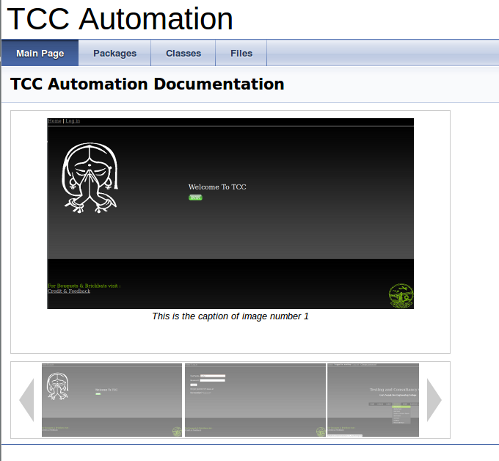
\includegraphics[scale=1.0]{doc.png}
\caption{Doxygen home page}
\end{figure}
\newpage
\begin{figure}[h]
\vskip 1cm
\centering 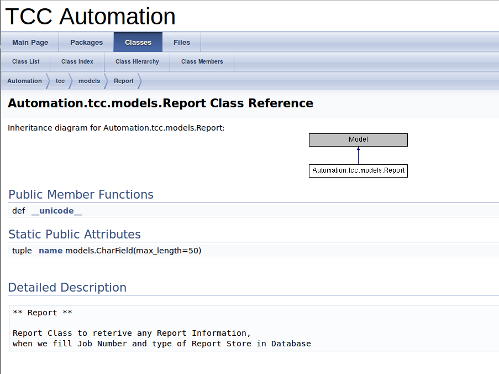
\includegraphics[scale=1.0]{doc3.png}
\caption{Documentation of models.py file}
\end{figure}
\newpage

\subsection{Shell Scripting}
{\bf What is Bash?}\\
Bash is a ``Unix shell": a command-line interface for interacting with the operating system. It is widely available, being the default shell on many GNU/Linux distributions and on Mac OS X; and ports exist for many other systems. It was created in the late 1980s by a programmer named Brian Fox, working for the Free Software Foundation. It was intended as a free-software alternative to the Bourne shell (in fact, its name is an acronym for "Bourne-again shell"), and it incorporates all features of that shell, as well as new features such as integer arithmetic and in-process regular expressions.\\\\
{\bf What is Shell ?}\\
The shell is the program which actually processes commands and returns output. Most shells also manage foreground and background processes, command history and command line editing. These features (and many more) are standard in bash, the most common shell in modern linux systems.\\\\
{\bf What is shell scripting?}\\
In addition to the interactive mode, where the user types one command at a time, with immediate execution and feedback, Bash (like many other shells) also has the ability to run an entire script of commands, known as a ``Bash shell script" (or ``Bash script" or ``shell script" or just ``script"). A script might contain just a very simple list of commands — or even just a single command — or it might contain functions, loops, conditional constructs, and all the other hallmarks of imperative programming. In effect, a Bash shell script is a computer program written in the Bash programming language.\\\\
Shell scripting is the art of creating and maintaining such scripts.\\\\
Shell scripts can be called from the interactive command-line described above; or, they can be called from other parts of the system. One script might be set to run when the system boots up; another might be set to run every weekday at 2:30 AM; another might run whenever a user logs into the system.\\\\
Shell scripts are commonly used for many system administration tasks, such as performing disk backups, evaluating system logs, and so on. They are also commonly used as installation scripts for complex programs. They are particularly suited to all of these because they allow complexity without requiring it: if a script just needs to run two external programs, then it can be a two-line script, and if it needs all the power and decision-making ability of a Turing-complete imperative programming language, then it can have that as well.\\\\
Some of the powerful commands used:
\begin{itemize}
\item SED : Sed is the ultimate stream editor, sed is a marvelous utility. Sed has several commands, but most people only learn the substitute command.
\item AWK : AWK is and important and excellent filter, and report writer.AWK is an excellent tool for processing these rows and columns, and is easier to use AWK than most conventional programming languages.
\end{itemize}
\newpage
Many features of shell scripting are also put to use :
\begin{itemize}
\item Functions.
\item Arrays.
\item Commands like sed, awk.
\item Use of mysql commands through shell-importing,exporting a database, etc.
\end{itemize}
\newpage

\subsection{Design}
{\bf System Design} : Systems design is the process or art of defining the architecture, components, modules, interfaces, and data for a system to satisfy specified requirements. One could see it as the application of systems theory to product development. There is some overlap with the disciplines of systems analysis, systems architecture and systems engineering.
\begin{enumerate}
\item  External design: External design consists of conceiving, planning out and specifying the externally observable characteristics of the software product. These characteristics include user displays or user interface forms and the report formats, external data sources and the functional characteristics, performance requirements etc. External design begins during the analysis phase
and continues into the design phase.
\item  Logical design: The logical design of a system pertains to an abstract representation of the data flows, inputs and outputs of the system. This is often conducted via modeling, which involves a simplistic (and sometimes graphical) representation of an actual system. In the context of systems design, modelling can undertake the following forms, including:
\begin{itemize}
\item Data flow diagrams
\item Entity Relationship Diagrams
\end{itemize}
\item  Physical design: The physical design relates to the actual input and output processes of the system. This is laid down in terms of how data is input into a system, how it is verified/authenticated, how it is processed, and how it is displayed as output.
\end{enumerate}
\newpage
{\bf Design Notations}:\\


Data Flow diagrams:

\begin{figure}[h]
\centering 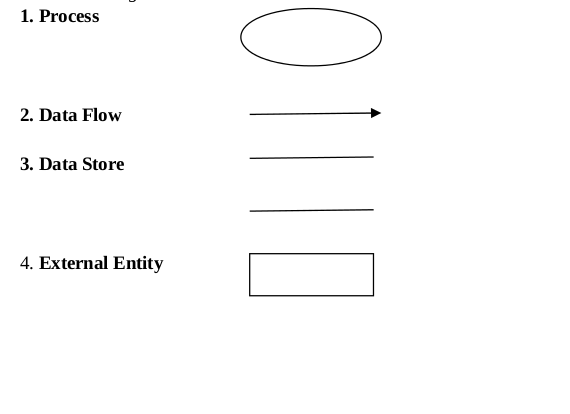
\includegraphics[scale=0.6]{sss1.png}
\end{figure}
Flow Charts:
\begin{figure}[h]
\centering 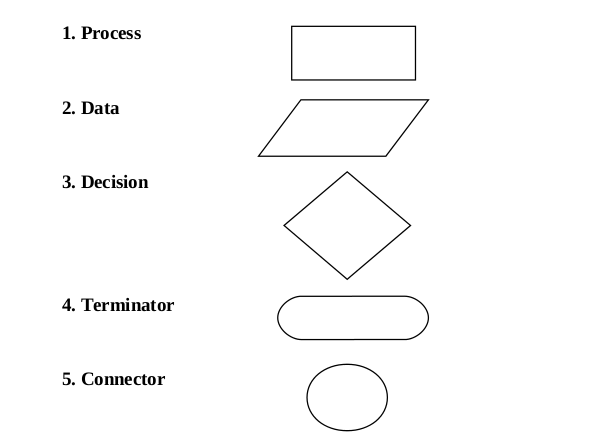
\includegraphics[scale=0.5]{sss2.png}
\end{figure}
\newpage
Entity Relationship Diagrams:\\
\begin{figure}[h]
\centering 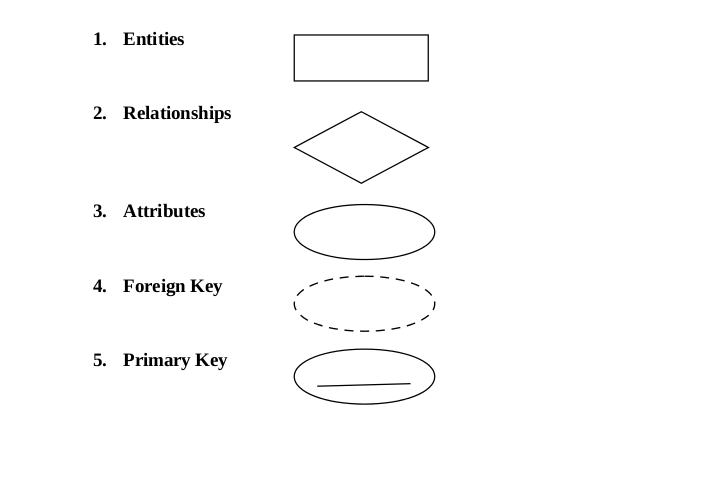
\includegraphics[scale=0.6]{sss3.png}
\end{figure}\\
 {\centering \bf Detailed Design}
We basically describe the functionality of the system internally. The internal design describes how data is
flowing from database to the user and how they both are internally connected. For this reason we can show
the design of the system in detailed manner by many ways:\\
{\bf Flowchart } A flowchart is a type of diagram that represents an algorithm or process, showing the steps as boxes of various kinds, and their order by connecting them with arrows. This diagrammatic representation can give a step-by-step solution to a given problem. Process operations are represented in these boxes, and arrows connecting them represent flow of control. Data flows are not typically represented in a flowchart, in contrast with data flow diagrams; rather, they are implied by the sequencing of operations. Flowcharts are used in analyzing, designing, documenting or managing a process or program in various fields



\newpage
\begin{figure}[h]
\centering 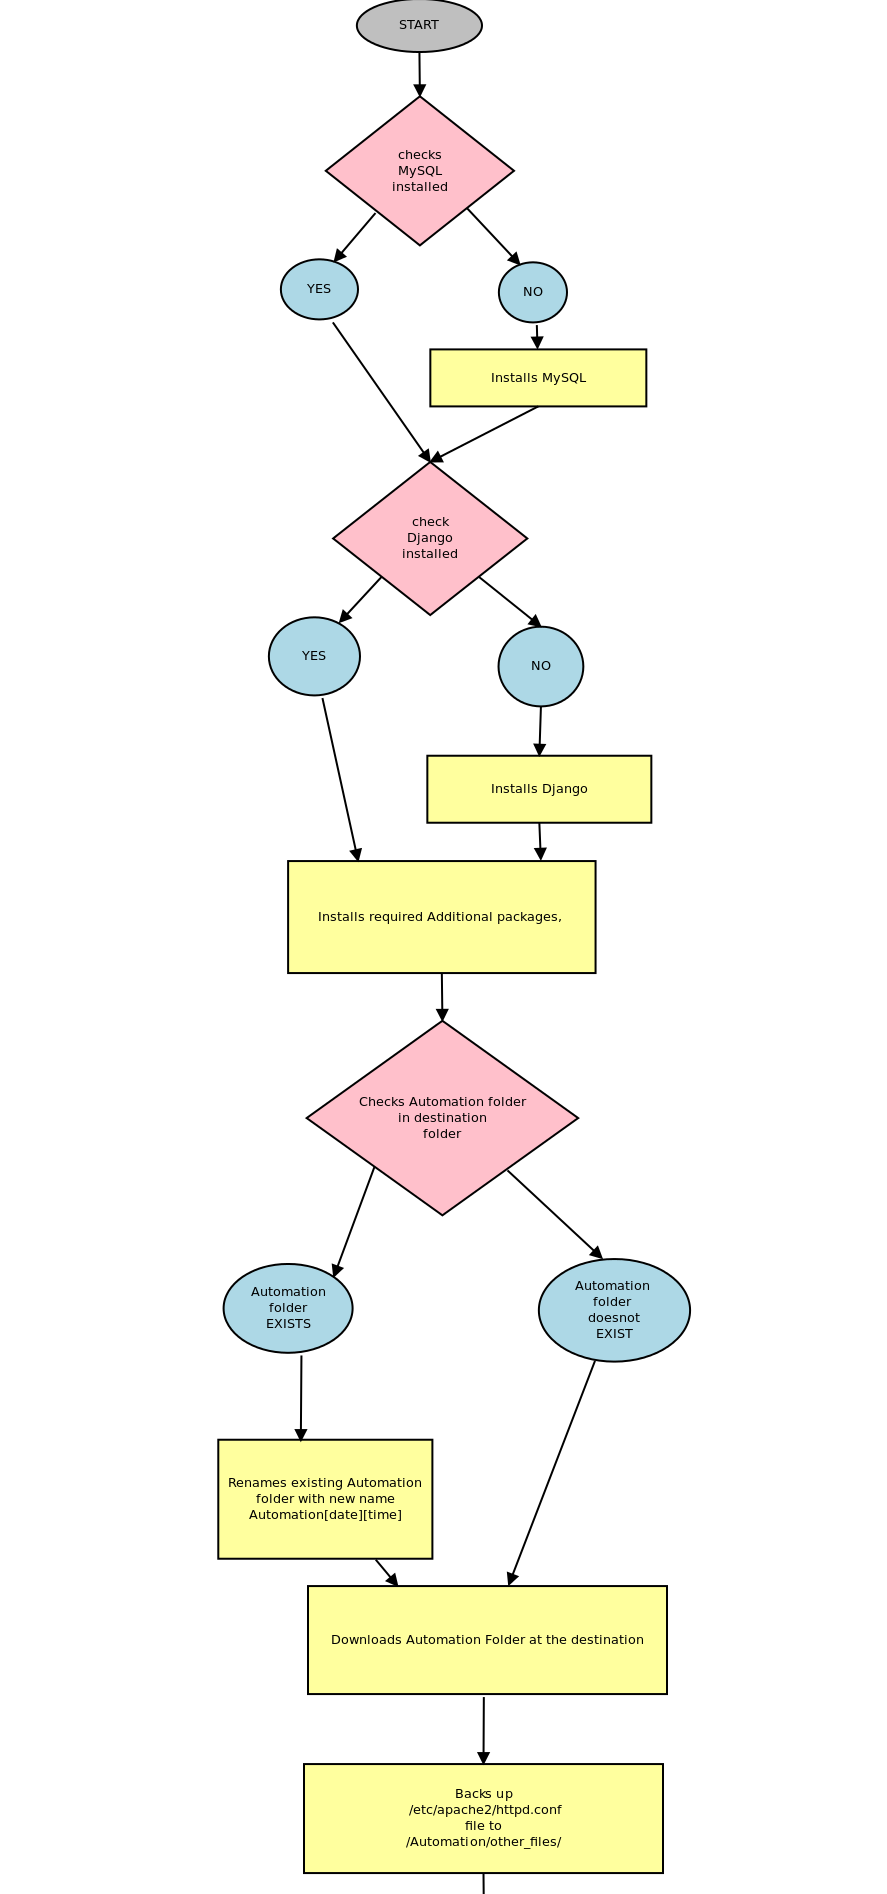
\includegraphics[scale=0.27]{inst1.png}
\end{figure}
\newpage
\begin{figure}[h]
\centering 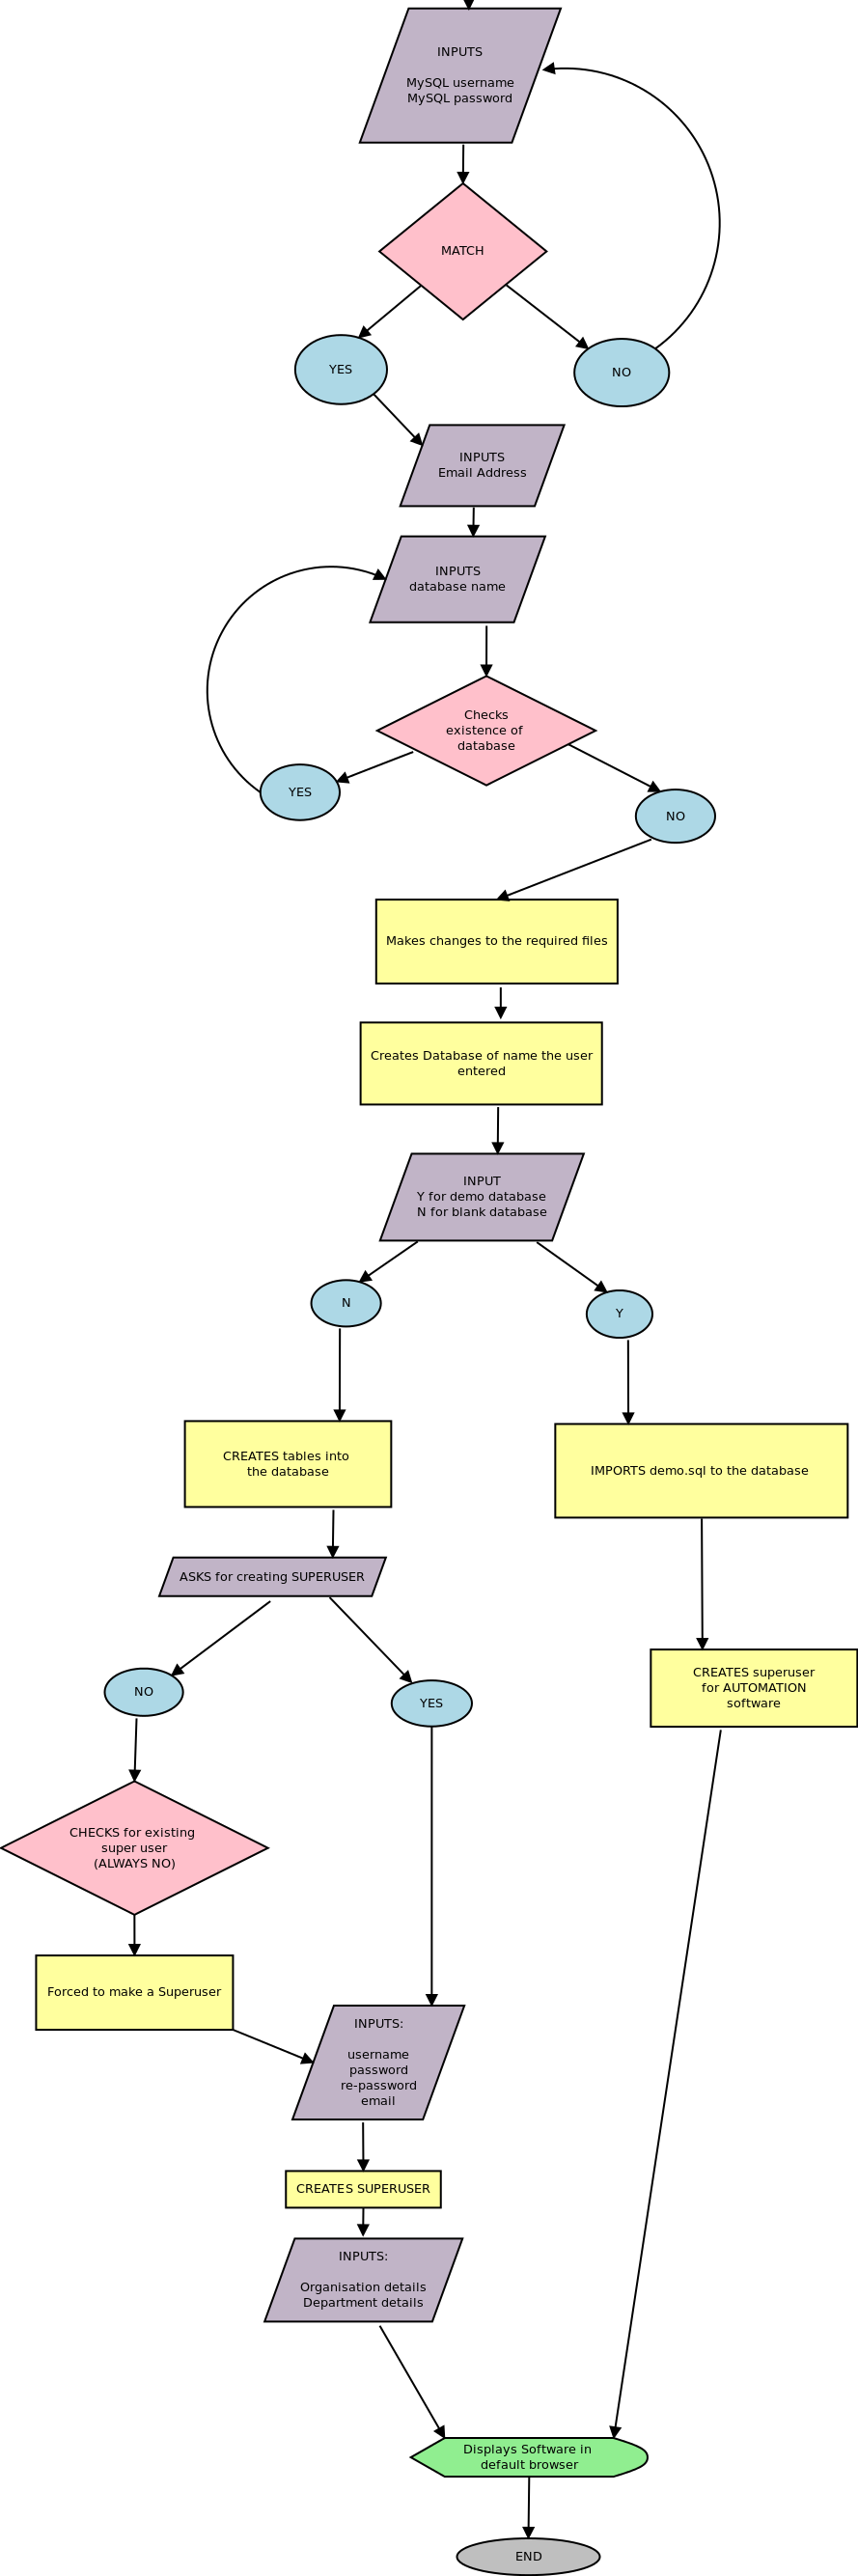
\includegraphics[scale=0.17]{inst2.png}
\caption{Flow Chart for Installation}
\end{figure}
\newpage
\begin{figure}[h]
\centering 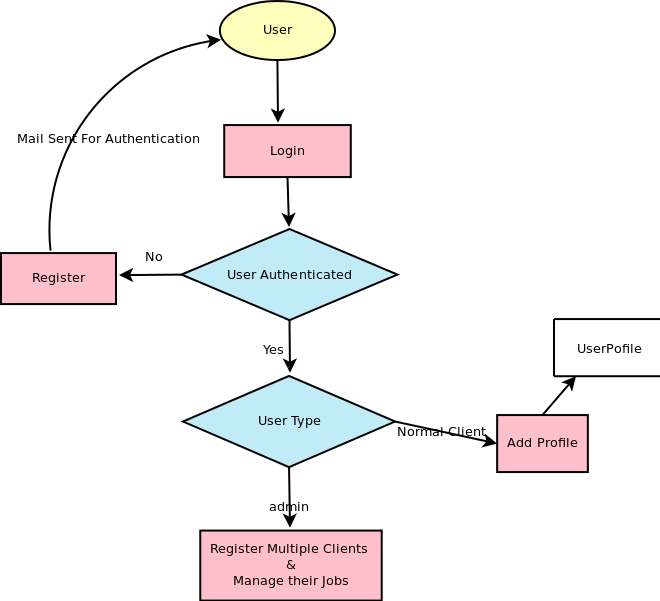
\includegraphics[scale=0.8]{register.png}
\caption{Flow Chart for Registeration}
\end{figure} 
\newpage
\begin{figure}[h]
\vskip 3cm
\centering 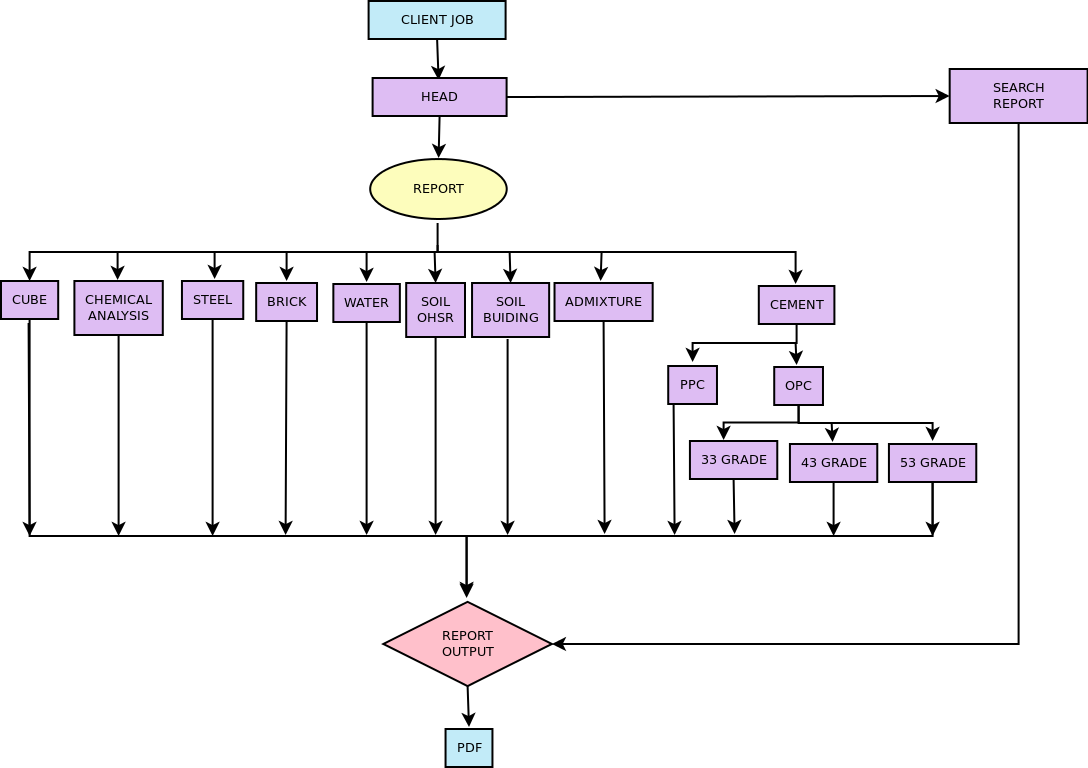
\includegraphics[scale=0.45]{report.png}
\caption{Flow Chart for Reports}
\end{figure} 
\newpage
\begin{figure}[h]

\centering 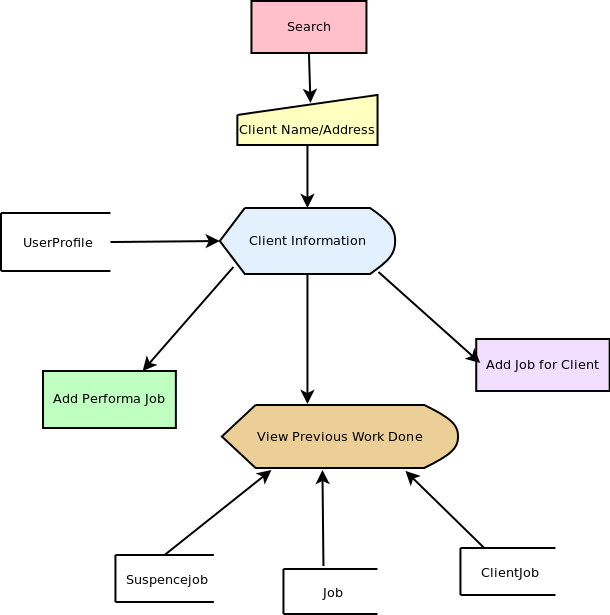
\includegraphics[scale=0.7]{search.png}
\caption{Flow Chart for Searching a Client}
\end{figure}

\newpage
\begin{figure}[h]
\centering 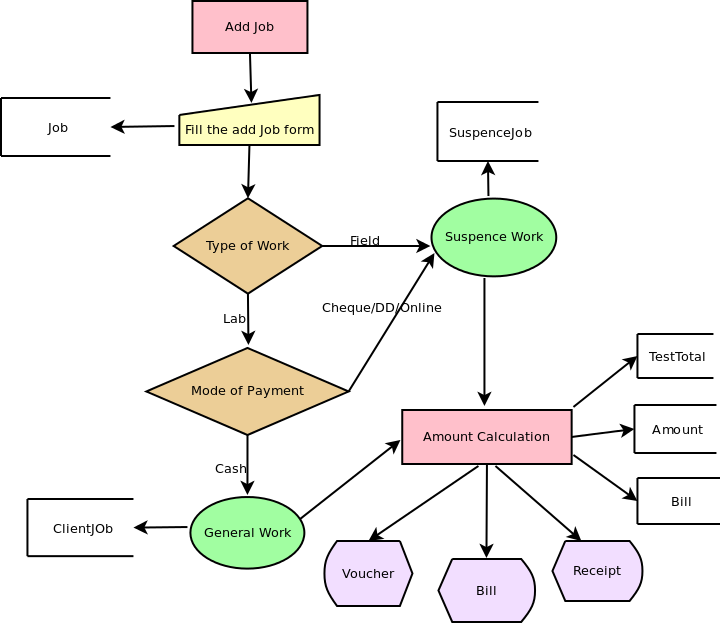
\includegraphics[scale=0.7]{addjob.png}
\caption{Flow Chart for adding a Job}
\end{figure}

\newpage
\begin{figure}[h]
\centering 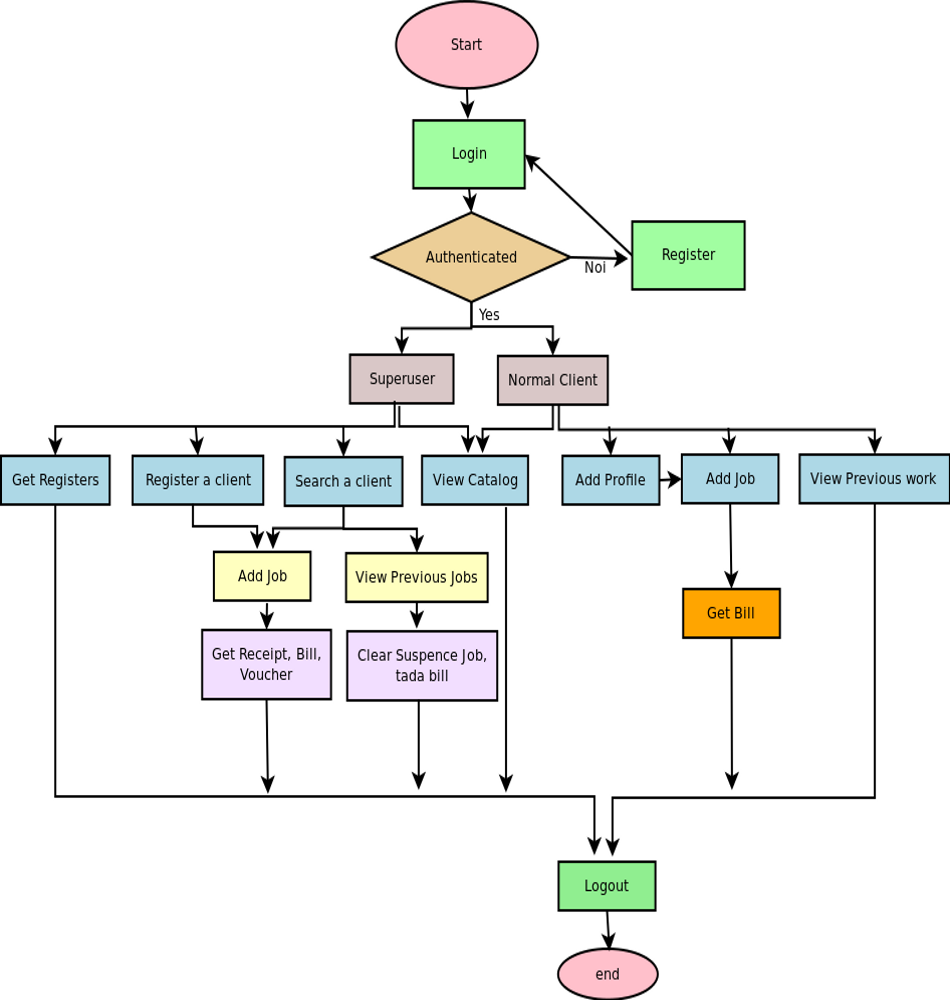
\includegraphics[scale=0.5]{automation.png}
\caption{Flow Chart for software}
\end{figure}
\newpage

{\bf Database Design}

\begin{figure}[h]
\centering 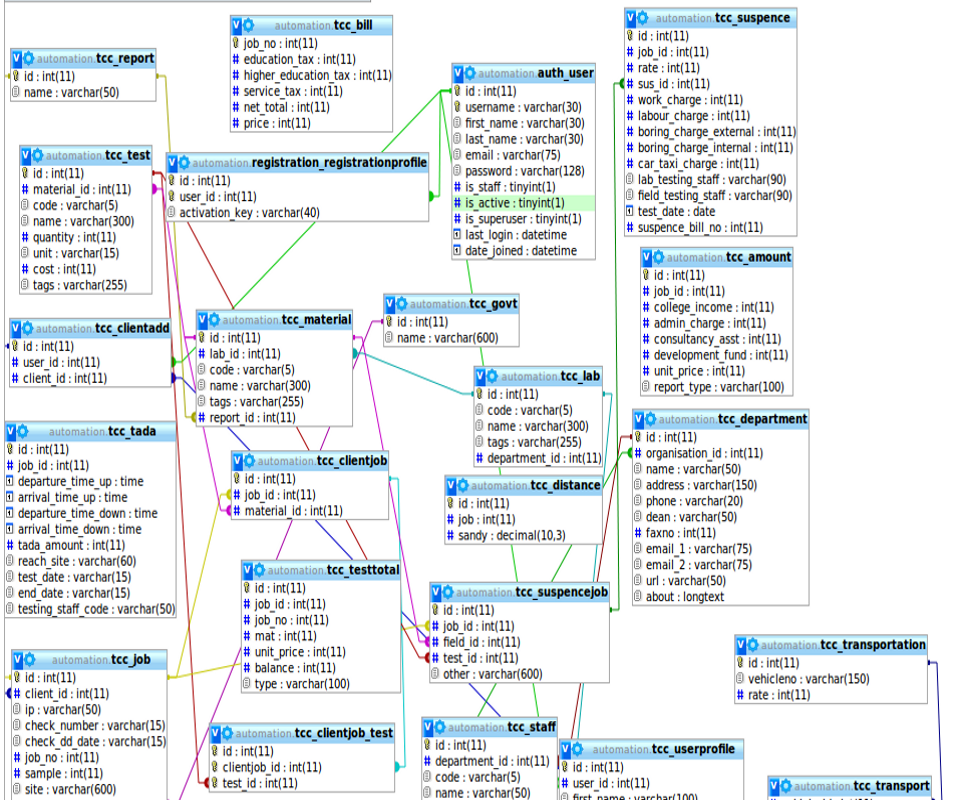
\includegraphics[scale=0.5]{db1.png}

\end{figure}
\newpage
\begin{figure}[h]
\centering 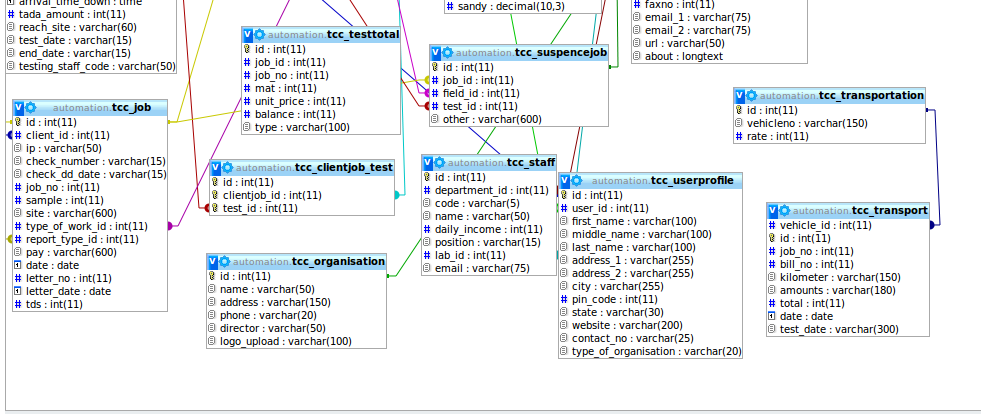
\includegraphics[scale=0.5]{db2.png}
\caption{Database Design}
\end{figure}
\newpage
\subsection{Introduction to TCC Automation Software}\\
Testing \& Consultancy Cell is a Department in our college that provide testing and Consultancy services to different clients. This cell does a lot of work like managing the clients, handling there work till completion. This work also requires managing a lot of paper work. Thus TCC Automation Software comes into the use. \\ 
{\bf Features of the Software}
\begin{itemize}
\item Open Source
\item User Interative Software
\item Online
\item Dynamic
\item Proper User and Admin interface
\item Catalog
\item Distance Calculation through map
\item Efficient Search module
\item Universal (Can be changed according to application/work)
\item Report generation
\item Single click installation
\item Proper User and develpor documentation
\end{itemize}
\newpage
\subsection{Modules of the Software}
\begin{description}
\item[1. Installation] : Installation of the Software and that too smoothly is the most important step for making the software run. The installation module is made, keeping in mind the different platforms or the versions of the system. The installation procedure is made very easy, informing the users about all the changes that are to be made in his/her system.
\item[2. Registration] : This involves user authentication, login, user Registration as a client. There are different views of the software that vaies on the user using it. That means user is able to see only that part to which he/she is authenticated.
\item[3. Catalog] : Catalog provides all the information about the product, there rate, quantity etc. Seeing the catalog list user can get an estimate of the total amount he would spend on entering a Job or work.
\item[4. Job Entry] : Job entry module involves entering the Job or work that need to be done in a particular lab or a site. This also involves getting the distance between the organisation and site. The client can add both Lab and Field works. Multiple works can be done in a single Job. 
\item[5. Amount Calculation] : Depending on the type of work to be done, material tested and number of tests to be performed the amount the automatically calculated by the Software. Then on the calculated amount the divisions are done and then taxes are applied.
\item[6. Search] : The search module include searching a client or Job that has previously been added. After getting the results of the search, the operations like getting the previous work done by the client, status of those works or further adding new works are performed. 
\item[7. Bill, Receipt \& Voucher Generation] : In this module after all the calculations done and data saved, the Bill, Receipt and the Voucher for the Job is generated that then is to be returned to the client.
\item[8. Registers Generation] : This module involves retrieving all the previous entries that were performed. These registeres include : Daily Report, Monthly Register, Main Register, Suspence Clearance Register, Lab Report, Client Report etc.
\item[9. CashBook] : CashBook module involve managing all the money transactions.  The involves all the cash debited or credited and the transactions made on them. 
\item[10. Reports Generation] : Report Generation module include generating the complete report for the field work.This gives the detailed information about the work done, staff mebers involved in doing the work, calculations done etc. Multiple Reports re generated for a work done from different labs. Once the report is generated one can download it too.
\end{description}
\newpage
\subsection{Automation Sofware in Detail}
{\bf Admin Interface}\\

The admin Interface is the Software interface for only admin. Using this interface admin can make all the changes in the Software. He/She is the utmost authority. The services that are given to the end user can be added, updated or deleted by the admin. Admin is the one who gives the permission for certain authority of a User.\\ 
\begin{figure}[h]
\centering 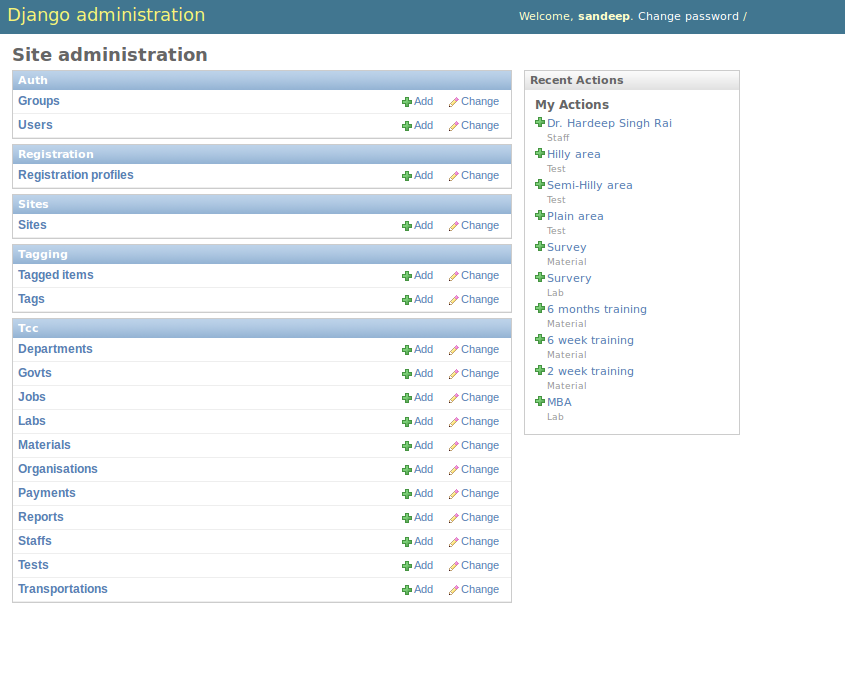
\includegraphics[scale=0.6]{admin.png}
\caption{Admin Interface}
\end{figure}

\newpage
{\bf Welcome Screen}\\

This Welcome Screen is visible as soon as the link to the Software is opened. This screen is visible to all the users even if they are authenticated or not.
\begin{figure}[h]
\vskip 2cm
\centering 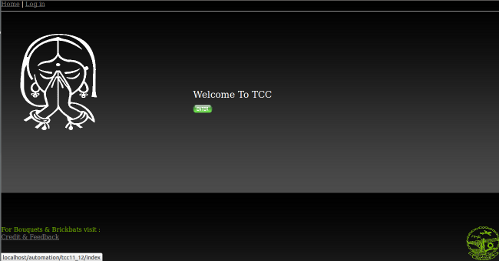
\includegraphics[scale=1.0]{welcome.png}
\caption{Welcome Screen}
\end{figure}

\newpage 
{\bf Registration \& Login}\\

When a User tries to login into the Software, the software checks, whethere the user is valid or is authenticated. If yes, the user login into the Software is susccesfull, else the User need to register himeself as the User.As soon as the user register himself, he will be sent an activation mail. In order to activate the account, the user has to open that link and login himself. Only the authenticated user is able to use the features of the software or work with it.
\begin{figure}[h]
\vskip 2cm
\centering 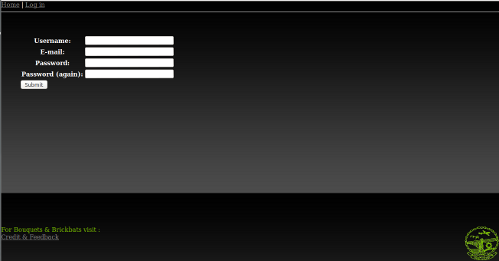
\includegraphics[scale=1.0]{register1.png}
\caption{Registration Screen}
\end{figure}

\newpage
{\bf Employee Login}\\
 
An employee is the User who has the authority to register other clients into the Software and then add there jobs or manage them. Once an authenticated employee login into the system, he/she is able to use all the fuctionality availble to him/her. He can add the clients, handle them, see the wotk of all the clients. A lot of features are availaber for the employer to automate his work and make it easy.
\begin{figure}[h]
\vskip 2cm
\centering 
\includegraphics[scale=1.0]{user1.png}
\caption{Employe Interface}
\end{figure}
\newpage
{\bf Normal User Login}\\

A normal User is considered as the client. He has very limited acess on the features of the software. In TCC Automation Software, the users have different web interface of the Software depending on the authority they are given. A normal User can have the information about all the services available, ask for a service, thus registering what actually he wants. He can also see the previous services he used from the Cell. 

\begin{figure}[h]
\vskip 2cm
\centering 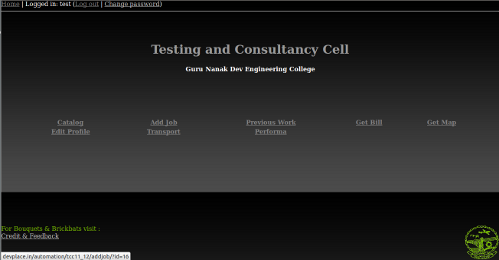
\includegraphics[scale=1.0]{user2.png}
\caption{Normal User Interface}
\end{figure}
\newpage
{\bf Catalog}\\
Catalog provides all the information about the product, there rate, quantity etc. Seeing the catalog list user can get an estimate of the total amount he would spend on entering a Job or work. A catalog represents a collection of products that you group into categories. You can then use this information to create, within a Commerce Server-enabled Web site, Web pages that let your customers browse your collection of products. The categories in your catalogs can have sub-categories, and products may appear in multiple categories.\\


\begin{figure}[h]
\centering 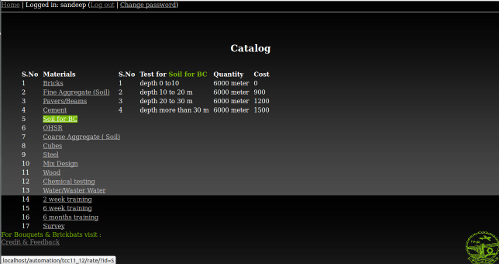
\includegraphics[scale=1.0]{Catalog.png}
\caption{Catalog}
\end{figure}\\

Catalogs contain hierarchies and relationships that you use to organize the products in the catalog to make it easier for customers to navigate to the products that they want to buy. You can create category hierarchies and relationships among categories and products that are in the same catalog or in different catalogs. For example, if you have a large catalog, you can create a parent category that includes several other categories, known as child categories. When customers navigate to the parent category, the child categories appear; enabling customers to navigate quickly to the category that contains the products they want.
\newpage
{\bf Add Job}\\

Both employee and Normal User can add the Job. The only difference is that an employee can add multiple jobs for his different clients and normal user can add the jobs for only himself. For adding the job one needs to fill all the necessary data required for a work to be done.
All the calculations about the amount for the Job is done in the backend. Only after you click the submit button you will be able to see the results.
\begin{figure}[h]
\vskip 2cm
\centering 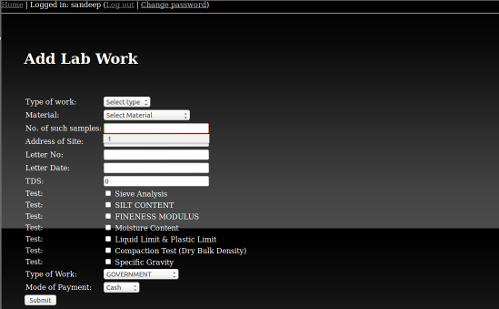
\includegraphics[scale=1.0]{addjob1.png}
\caption{Add Job Form}
\end{figure}

\newpage
{\bf Search Module}\\

The search module include searching a client or Job that has previously been added. After getting the results of the search, the operations like getting the previous work done by the client, status of those works or further adding new works are performed. It is an important feature of the software as it keeps the track of the clients getting services from the organisation.

\begin{figure}[h]
\vskip 2cm
\centering 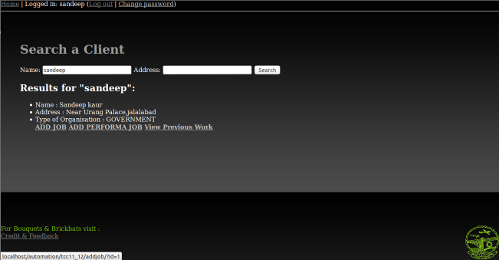
\includegraphics[scale=1.0]{search1.png}
\caption{Search Module}
\end{figure}\\

In this, the Software looks for the certain keyword you entered in the corresponding table. The filteration is done and those results with matching keywords are listed. 

\newpage
{\bf Bill, Receipt \& Voucher generation}\\

Once the Job is entered into the software, irrespective of when it will start, the client is required to make the payment. After that he is given the Receipt and bill for his work. The Bill, Receipt and Voucher are automatically generated only after a complete and valid Job is added into the software.
\begin{figure}[h]
\vskip 2cm
\centering 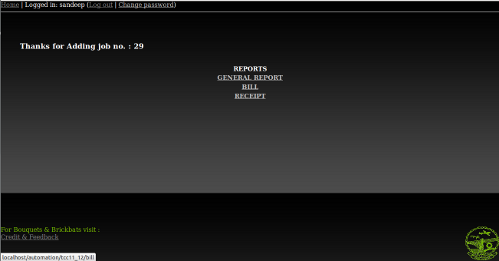
\includegraphics[scale=1.0]{Bill.png}
\caption{Get Bill, Receipt \& Voucher}
\end{figure}

\newpage 
{\bf Registers Generation}\\

This module involves retrieving all the previous entries that were performed. These registeres include : Daily Report, Monthly Register, Main Register, Suspence Clearance Register, Lab Report, Client Report etc. For getting different registers diffeent queries are performed or filter are applied, depending on the need.\\
\begin{figure}[h]
\centering 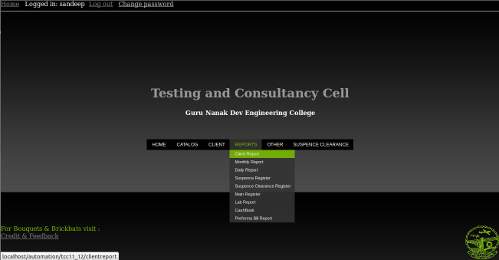
\includegraphics[scale=1.0]{registers.png}
\caption{Select the Register}
\end{figure}\\
{\bf Registers generated in the software}\\
Following are the reports generated in TCC Automation software :
\begin{itemize}
\item Suspence Report: This report keep record of all the suspence jobs that has been registered.
\item Suspence-Clearance Report: This report is used to get all te suspence registered jobs whose dues have been cleared out.
\item T.A./D.A. Bill: This is report for Transport Allowance and Daily Allowance bill.
\item Performa Bill: It give the 
\item Job Register: It keep record of all the jobs registered.
\item Yearly/Monthly Income Report: It gives the yearly and monthly record of income to the institute.
\item Transport Bill: It gives all the information related to transportation.
\item Other charge Bill: It gives the report of all the other charges like service tax, education tax, etc.
\item Daily report: It gives the information of job registered in  the number of days selected. It also makes the differance between the types of payments made like cheque, cash.
\item Faculty Income distribution: It keeps the record of the income distribution to the faculty members.
\item Main Register: It is the main register keeping the record of all the report types.
\item Receipt: It keeps te record of all the recieps. One only need to know the job no. and then can easily get the receipt.
\item Department/lab Report: It carries all the information of various labs and thus gives the record for the lab selected.
\item Govt./Semi-Govt./Private Report: It keeps the record for the type of work selected i.e Govt./Semi-Govt./Private Report.
\item Clearance Report: It gives the clearance report.
\item General Bill: It keeps record of all the general reports.
\end{itemize}

\begin{figure}[h]
\centering 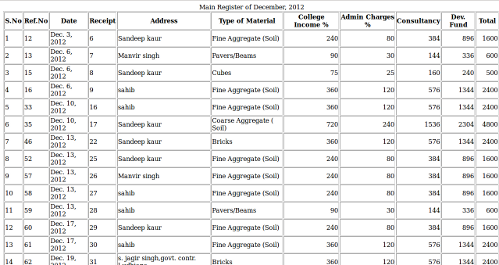
\includegraphics[scale=1.0]{reg1.png}
\caption{Output Register}
\end{figure}

\newpage
{\bf Report Generation}\\

Report Generation module include generating the complete report for the field work.This gives the detailed information about the work done, staff mebers involved in doing the work, calculations done etc. Multiple Reports re generated for a work done from different labs. Once the report is generated one can download it too. Now the basic requirement of the project  is to produce the report from the the data which were submitted by the user or client in the office for the testing purpose. So, for that we require the generic views for the software to display the data from the models of the report and to display that data to the user we also need the templates for the different types of the reports. It is necessary for the report application that the templates for the report application must be different from the other application templates so that it is easily distinguished from the tcc application which was another application in the project. So, for this purpose the different template inside the templates of the project was made to distinguish the different template. This template is known as ``report".\\\\
The reports are generated from the models which are predefined in the models of the report application, In the  models field, there are different types of field which are responsible for storing the data in the different datatypes. The good thing is that we can distinguish between the tables of the two applications very easily, as the prefix for the different applications are set by default by the the syncdb process. And in this case, the models are made with the prefix ``report".\\\\
\begin{figure}[h]
\centering \includegraphics[scale=1.0]{3.png}
\caption{Types of Report}
\end{figure}
SELECTING THE TYPE OF REPORT FROM THE GIVEN MATERIAL :\\\\
To make the report one should need to select the type of report which the user want to produce, so for this purpose the report type has to be chosen from the list of the available report in the software. The report formats are directly called from the models via views and a common form.html is responsible for displaying the form.\\\\
On clicking any of the report the specific report is selected and we can proceed further to fill the entries into that report.\\\\
SELECTING AND MAKING A SPECIFIC REPORT TYPE\\\\
At this step, the selected report form is displayed in front of the user and now the user can fill the data which he can attain from the lab after testing the different material, there might be the different samples of the same material, at the top of the form a column for specifying the sample no is given in the form, the form them contains the different fields according to the requirement of the material and test. All the fields are predefined according to the different tests, so the user only have to fill the test values in the form.\\\\
FINAL REPORT\\
The final report is produced by clicking on the submit button on the form in the report type to be added. The sample of the report is attached below: 
\newpage
\begin{figure}[h]
\centering 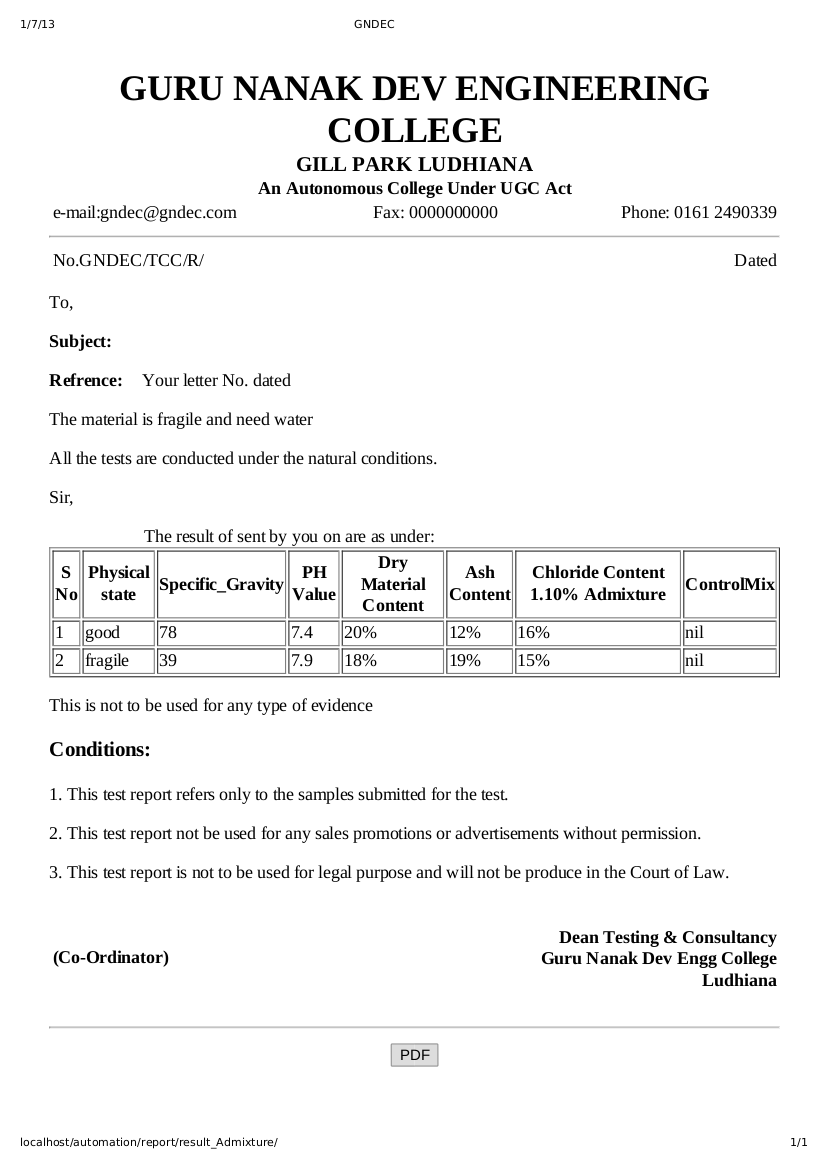
\includegraphics[scale=0.5]{GNDEC.png}
\caption{Report Generated}
\end{figure}




\newpage
{\bf Distribution of money}\\

\begin{itemize}
\item College Income
\item Administrative
\item Development Funds
\item Consultatancy Asst.
\item Service Tax
\item Education Tax
\item Higher-Education Tax
\end{itemize}
\newpage
\subsection{Testing}
Project testing is an investigation conducted to determine the quality of the project and the services
provided by the project. Testing is the process of analyzing a project to detect the differences between
existing and required conditions (that is defects/errors/bugs) and to evaluate the features of the project.
After complete development of the project it is mandatory to test the project.
The main motive of the project testing is to identify whether project is able to meet user requirements or
not. To know the better performance of project we have to develop various Test Cases. Now, designing
good test cases is a complex art. The complexity comes from three sources:
\begin{enumerate}
\item Test cases help us discover information. Different types of tests are more effective for
different classes of information.
\item Test cases can be “good” in a variety of ways. No test case will be good in all of them.
\item Our tend to create test cases according to certain testing styles, such as domain testing or
risk-based testing. Good domain tests are different from good risk-based tests.
\end{enumerate} 
\newpage
\subsection{Implementation}
Implementation is the process of converting a new or revised system design into an operational one. At the
present time there is no system as Imperial Finance which work online and provide information via web.
So this is the replacement of the manual financial system. In Imperial Finance most of the finance related
task will be performed online.\\\\
Types of Implementation:
\begin{enumerate}
\item Implementation of a computer system to replace a manual system.
\item Implementation of a new computer system to replace an existing one.
\item Implementation of a modified application to replace an existing one.
\end{enumerate}
\vskip 0.5cm
Aspects of Implementation:
\begin{enumerate}
\item Conversion
\item Post Implementation and review
\item Software maintenance
\end{enumerate}
\vskip 0.5cm
{\bf Implementation of the Project }:\\
TCC Automentation Software is the implementation of the with the new one. The current software is offline without any registration module thus making the management of clients and there data difficult. There is no search module. Thus when there is a need to search a client or a job, the employee need to go to the backend and see the database. This process
is very time consuming and irritating. The project implementation of Imperial Finance starts with the
Administrator. Administrator will be the super user of the application who will configure system
information such as new services, lab, employees and new clients. There will be a different
interface for the employees and clients from where they can manage and view the TCC related
information which they allowed to view.\\
It is a web based application, so it is distributed and data centric. In this application, MySQL database is
used to store data related to employees, users offered by system, clients, etc. Since database is on Server,
so any number of users can work simultaneously and can share their data with each other.\\\\
{\bf Conversion Plan}:\\
Conversion is the process of changing from one system to another. This plan involves:
\begin{enumerate}
\item Creating computer-compatible files.
\item Training the operating staff.
\item Installing terminals and hardware.
\end{enumerate}
\newpage
{\bf Conversion Processes} :
\begin{enumerate}
\item File Conversion.
\item  Data Entry.
\item User Training.
\end{enumerate}
\vskip 0.5cm
{\bf Elements of User training} :
\begin{enumerate}
\item The initial training period.
\item At the time of Installation.
\item If required, during Maintenance Phase.
\end{enumerate}

\newpage
\subsection{Post-Implementation and Software Maintenance}
implementation review is an evaluation of a system in terms of the extent to which the system
accomplishes stated objectives and actual project costs exceeds initial estimates.\\\\
{\bf Review Plan}: An overall plan covers,\\
\begin{enumerate}
\item Administrative plan.
\item Personnel requirements plan.
\item Hardware plan.
\item Documentation review plan.
\end{enumerate}
\vskip 0.5cm
After the implementation of this project, the team will see the post implementation phase. If there will be
any concerns, those will be solved based on the user feedback.\\\\
{\bf Maintenance} : In order for a software system to remain useful in its environment it may be necessary to
carry out a wide range of maintenance activities upon it. There are bugs to fix, enhancement to add and
optimization to make, changes has to be done in older version to make it application for current use of
current version to cater the need of future. Maintenance can be of three types: -\\
\begin{enumerate}
\item Corrective Maintenance: Changes necessitated by actual errors (defects or residual "bugs") in a
system are termed corrective maintenance. These defects manifest themselves when the system does not
operate as it was designed or advertised to do. A defect or “bug” can result from design errors, logic errors
and coding errors. Design errors occur when for example changes made to the software are incorrect,
incomplete, wrongly communicated or the change request misunderstood. In the event of a system failure
due to an error, actions are taken to restore operation of the software system. The approach here is to
locate the original specifications in order to determine what the system was originally designed to do.
\item Adaptive Maintenance: Any effort that is initiated as a result of changes in the environment in which
a software system must operate is termed adaptive change. Adaptive change is a change driven by the need
to accommodate modifications in the environment of the software system, without which the system
would become increasingly less useful until it became obsolete. The term environment in this context
refers to all the conditions and influences which act from outside upon the system, for example business
rules, government policies, work patterns, software and hardware operating platforms. A change to the
whole or part of this environment will warrant a corresponding modification of the software.
\item Perfective Maintenance: This is actually the most common type of maintenance encompassing
enhancements both to the function and the efficiency of the code and includes all changes, insertions,
deletions, modifications, extensions, and enhancements made to a system to meet the evolving and/or
expanding needs of the user. A successful piece of software tends to be subjected to a succession of
changes resulting in an increase in its requirements. This is based on the premise that as the software
becomes useful, the users tend to experiment with new cases beyond the scope for which it was initially
developed. Expansion in requirements can take the form of enhancement of existing system functionality
or improvement in computational efficiency. Though efforts have been made to develop error free
systems, but no system is perfect, room for improvement is always there. Thus proper documentation for
the system has been done so that it will be easy to handle any breakdown or any other type of system
maintenance activity.





\newpage
\section{About My Project}
\subsection{Reports generated in the software}
Following are the reports generated in TCC Automation software :
\begin{itemize}
\item {\bf{ Suspence Report:}} This report keep record of all the suspence jobs that has been registered.
\item {\bf{Suspence-Clearance Report:}} This report is used to get all te suspence registered jobs whose dues have been cleared out.
\item {\bf {T.A./D.A. Bill:}} This is report for Transport Allowance and Daily Allowance bill.
\item {\bf {Performa Bill:}} It give the 
\item {\bf {Job Register:}} It keep record of all the jobs registered.
\item {\bf {Yearly/Monthly Income Report:}} It gives the yearly and monthly record of income to the institute.
\item {\bf {Transport Bill:}} It gives all the information related to transportation.
\item {\bf {Other charge Bill:}} It gives the report of all the other charges like service tax, education tax, etc.
\item {\bf {Daily report:}} It gives the information of job registered in  the number of days selected. It also makes the differance between the types of payments made like cheque, cash.
\item {\bf {Faculty Income distribution:}} It keeps the record of the income distribution to the faculty members.
\item {\bf {Main Register:}} It is the main register keeping the record of all the report types.
\item {\bf {Receipt:}} It keeps te record of all the recieps. One only need to know the job no. and then can easily get the receipt.
\item {\bf {Department/lab Report:}} It carries all the information of various labs and thus gives the record for the lab selected.
\item {\bf {Govt./Semi-Govt./Private Report:}} It keeps the record for the type of work selected i.e Govt./Semi-Govt./Private Report.
\item {\bf {Clearance Report:}} It gives the clearance report.
\item {\bf {General Bill:}} It keeps record of all the general reports.
\end{itemize}
\newpage
\begin{figure}[h]
\centering \includegraphics[scale=0.7]{a1.png}
\caption{Bill Report}
\end{figure}
\newpage
\begin{figure}[h]
\centering \includegraphics[scale=0.7]{a2.png}
\caption{General Clearance Report}
\end{figure}
\newpage
\begin{figure}[h]
\centering \includegraphics[scale=0.7]{a3.png}
\caption{Suspense Clearance Report}
\end{figure}
\newpage


\subsection{Distribution of money}
\begin{itemize}
\item College Income
\item Administrative
\item Development Funds
\item Consultatancy Asst.
\item Service Tax
\item Education Tax
\item Higher-Education Tax
\end{itemize}
\newpage
\subsection{My Contribution to the project}
\begin{itemize}
\item Made Login and registration application
\item Added a report named `Daily Report'
\item Added a module named `Labs'
\item Introduced new tables in admin section
\item Gave different database permissions to different staff members\\
\end{itemize}

\newpage
\begin{description}
\item[Login Application] : This application allows one register oneself in the software and use it by logging in. This increased the security of the project as now only the authorised users can have access to the software and thus use it. Any unauthorised user now cannot misuse it.
\end{description}
\begin{figure}[h]
\centering 
\includegraphics[scale=0.3]{Screenshot.png}
\caption{Login application introduced in software}
\end{figure}
\newpage
\begin{description}
\item[Daily Report module] : It was not possible earlier to have a record amount of a day in TCC or number of number of days selected but after introduction of this module in the software one can do so. This has moreover increased the level of automation.
Also it can make the differanc between the type of payment made. That means now on can have record of cash and cheques payments making the users easy to handle the work.
\end{description}


\begin{figure}[h]
\centering \includegraphics[scale=0.4]{s1.png}
\caption{Daily Report module added}
\end{figure}
\begin{figure}[h]
\newpage
\centering 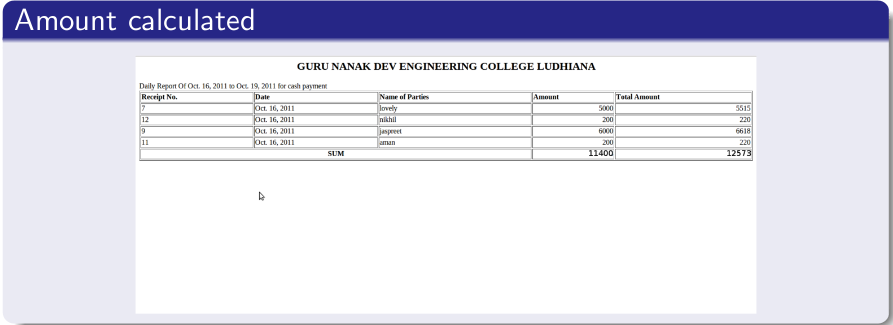
\includegraphics[scale=0.4]{dp3.png}
\caption{Cash type selected to make selection for report}
\end{figure} 
\begin{figure}[h]
\centering 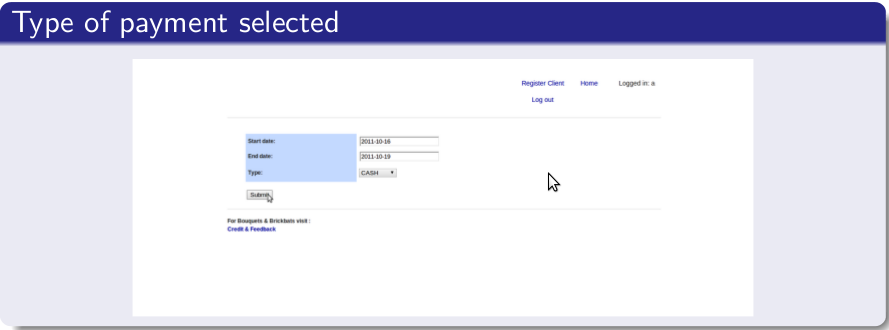
\includegraphics[scale=0.4]{dp4.png}
\caption{Report for cash payment for number of days selected}
\end{figure} 
\begin{description}
\newpage
\item[Labs module] : This module is used to find the amount recieved for a particular lab for the number of days selected. It gives the record for the labs in TCC for number of days selected. It has also automated the work.
\end{description}
\begin{figure}[h]
\centering \includegraphics[scale=0.4]{s4.png}
\caption{labs module added}
\end{figure}
\newpage
\vspace{5cm}
\begin{figure}[h]
\centering 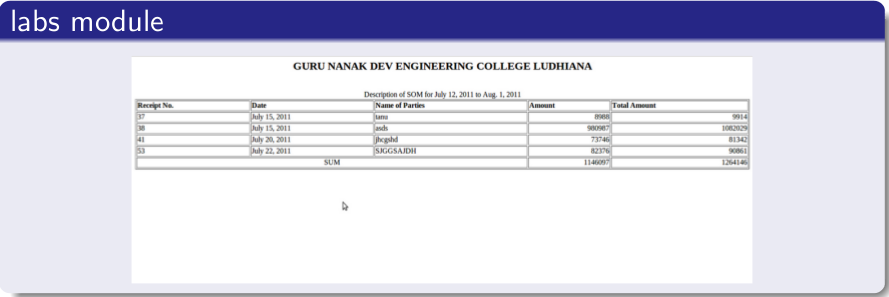
\includegraphics[scale=0.4]{lb1.png}
\caption{Amount recieved for the lab in number of days selected}
\end{figure}
\newpage
\begin{description}
\item[Introduction of new tables in admin] : Introduction of new tables in admin has made the admin of software more powerful as now in order to change the database entries he can directly make changes by going to these tables. This made the interface of user with the software easier, without getting tracked in the datbase tables and codings.
\end{description}
\begin{figure}[h]
\centering 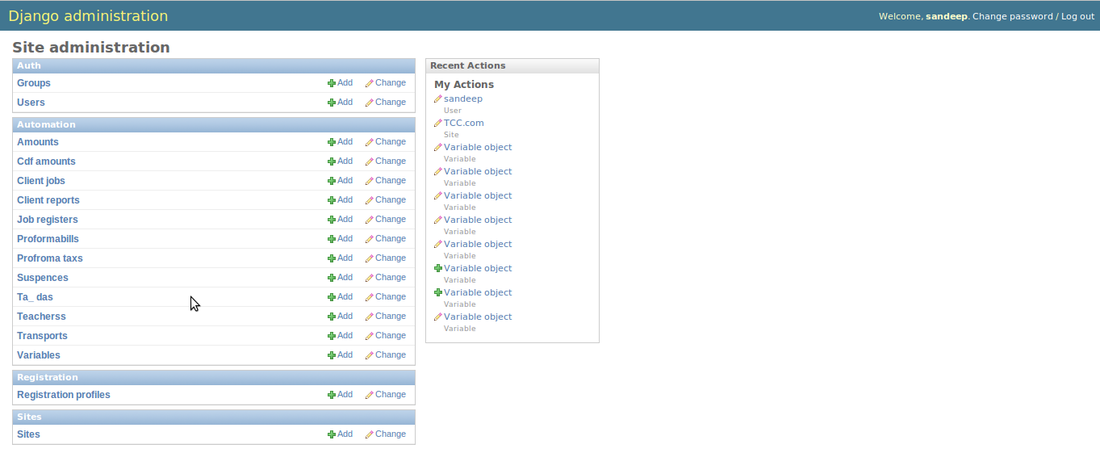
\includegraphics[scale=0.4]{s5.png}
\caption{Automation tables added in admin}
\end{figure}
\newpage
\subsection{Advantages of Automation}
\begin{itemize}
\item Great way to save money.
\item Reduce paper work.
\item Automatic calculations.
\item Less man power.
\item Increased efficiency.
\item Increased Accuracy.
\item Less time for protecting information.
\item Handle a work more faster.
\item Backup record.
\item Easy transformation.
\item Easy management.
\item Less storage space is required.
\item Overall development of system.
\item Minimize error and processing.
\end{itemize}


                               %% More section can be added as per requirement


%-------------------------------------------------------------
\include{bibliography} 		%Referrences
%------------------------------------------------------------------------


\end{document}
%%------------------------End document-------------------------%%
